% ASPLOS 2027 submission format: use \documentclass[sigplan,anonymous,review,nonacm]{acmart}
% when compiling with texlive/pdflatex. Tectonic has a known hyperref compatibility issue.
% Current format: IEEEtran for development and proofreading.
\documentclass[conference]{IEEEtran}

\usepackage[T1]{fontenc}
\usepackage{cite}
\usepackage{amsmath,amssymb,amsfonts}
\usepackage{array}
\usepackage{booktabs}
\usepackage{graphicx}
\usepackage{microtype}
\usepackage{textcomp}
\usepackage{pifont}
\usepackage{xcolor}
\usepackage{tikz}
\usepackage{url}

\usetikzlibrary{arrows.meta,calc,positioning}

\newcolumntype{P}[1]{>{\raggedright\arraybackslash}p{#1}}

\definecolor{envred}{HTML}{E56B6F}
\definecolor{envblue}{HTML}{4D7EA8}
\definecolor{envgreen}{HTML}{5AA469}
\definecolor{envcyan}{HTML}{4EA5A0}
\definecolor{envorange}{HTML}{E6A157}
\definecolor{envyellow}{HTML}{E9C46A}
\definecolor{envgray}{HTML}{D9DCE3}
\definecolor{envdark}{HTML}{233142}
\definecolor{envlight}{HTML}{F7F8FA}

\tikzset{
stage/.style={
	rounded corners=6pt,
	draw=envdark,
	line width=0.5pt,
	align=center,
	inner sep=6pt,
	minimum height=10mm,
	font=\scriptsize
},
flowarrow/.style={-{Latex[length=2.2mm,width=1.7mm]}, line width=0.7pt, draw=envdark},
paneltitle/.style={font=\bfseries\scriptsize, text=envdark},
callout/.style={font=\scriptsize, text width=0.86\columnwidth, align=center, text=envdark}
}

\begin{document}

\title{Beyond Strict Prefix Caching for Structured LLM Serving}

\author{\IEEEauthorblockN{Anonymous Authors}}

\maketitle

\begin{abstract}
Modern LLM serving systems reuse cached KV state for shared token prefixes, but structured workloads---agent pipelines, tool-augmented workflows, semi-templated enterprise traffic---routinely place a short dynamic envelope in front of a long stable body, defeating front-aligned prefix matching. We show that in such workloads strict prefix reuse covers only 17.4\% of prompt tokens while exact structural reuse reaches 77.9\%, and that most of this gap is recoverable without general segment composition. We formalize \emph{body reuse}: a request splits into a fresh envelope~$E$ and an exact reused body~$B$. We argue that the $E \Vert B$ ordering is a correctness requirement enforced by rotary position embeddings: reordering to $B \Vert E$ (the approach of Lumer et al.) changes cross-segment attention patterns and produces different outputs, making it impermissible as a transparent serving optimization. Under this constraint, body reuse is the only known mechanism that reuses body KV state across requests while preserving bit-exact outputs. The runtime accepts an envelope hint at the API surface and commits a two-span prefill plan that prefills only~$E$ while attaching body KV blocks from a content-addressed registry. Evaluated on a 32B-parameter model deployed on production NPU hardware with tensor parallelism (TP=2), body reuse delivers \textbf{+120\%} request throughput and \textbf{--75\%} mean TTFT over the stock serving baseline under production-realistic body reuse (8.3 requests per unique body), while producing bit-exact outputs. Under a worst-case stress test with 60 unique bodies, the mechanism degrades gracefully to baseline performance.
\end{abstract}

\begin{IEEEkeywords}
large language model serving, prefix caching, KV cache reuse, segment reuse, prompt structure, runtime systems
\end{IEEEkeywords}

\section{Introduction}

Online LLM serving has matured around several core systems ideas: continuous batching for accelerator utilization~\cite{yu2022orca}, careful KV-cache memory management for larger working sets~\cite{kwon2023efficient}, and faster attention kernels for lower decode overheads~\cite{dao2022flashattention,dao2023flashattention2}. These advances substantially improve throughput and latency, but they leave open a different systems question: what reusable prompt structure is still invisible to the reuse abstraction used by the runtime?

Recent empirical studies of prompt caching for agentic workloads directly expose this fragility. Lumer et al.~\cite{lumer2026dontbreak} evaluate prompt caching across four flagship LLMs (GPT-4o, GPT-5.2, Claude Sonnet~4.5, Gemini~2.5~Pro) on long-horizon agentic tasks with 10{,}000-token system prompts. Their no-cache baseline prepends a short UUID to the system prompt---a few tokens of dynamic content in front of a large stable body---and completely defeats prefix caching, forfeiting 45--80\% cost savings and 6--31\% TTFT improvement. They identify this as the dominant deployment pattern: session identifiers, routing headers, and timestamps naturally precede the stable system prompt in agent frameworks. Pan et al.~\cite{pan2025kvflow} further show that even with static agent prompts, standard LRU eviction policies cause cache misses in multi-agent workflows because agents cycle through execution order. Both studies converge on the same structural observation: when a short dynamic prefix precedes a long stable body, the prefix-first reuse abstraction silently discards the dominant reusable unit.

Today, most production-grade reuse mechanisms remain prefix-first. A request can skip prefill only when previously materialized KV state corresponds to an exact front-aligned token prefix. This works well for rigid templates, but it is too weak for structured serving workloads in which requests are assembled from reusable prompt objects such as system instructions, tool manifests, memory summaries, policy blocks, and domain context. In these workloads, a short dynamic envelope often sits in front of a long stable body. Once the envelope changes, a strict-prefix cache loses visibility into the repeated body behind it.

The issue is not that prefix caching is slow or unimportant. The issue is that strict prefix matching no longer represents the dominant exact reusable unit in modern structured traffic. A serving engine can report healthy prefix reuse while still recomputing the prompt tokens that dominate prefill cost and KV footprint. This is especially visible in agent and workflow prompts, where repeated bodies are exact and large, but front-most routing, user, or task headers vary from request to request.

This paper identifies that mismatch and asks a narrower systems question than generalized segment composition. If one preserves exact token identity and realistic serving semantics, how much reusable prompt structure lies beyond the strict prefix boundary, and what is the smallest exact mechanism that must be implemented before any end-to-end online gain claim is justified? We do not begin with approximate matching, semantic retrieval, or embedding-based heuristics. We ask instead whether structured serving needs a different exact reuse unit and, if so, how small the first deployable runtime mechanism can be.

A critical constraint shapes this question. Cache-boundary control~\cite{lumer2026dontbreak}---the strongest existing approach---reorders the prompt to $B \Vert E$, making the body front-aligned for prefix caching. We argue that this reordering is \emph{impermissible} as a transparent serving optimization: under RoPE~\cite{su2021roformer}, swapping the envelope and body changes the absolute position of every token, which changes cross-segment attention weights and produces provably different model outputs. A cache optimization must not alter the computation the model performs. The $E \Vert B$ ordering is therefore a correctness requirement, not a convention. Under this constraint, the only way to reuse body KV state across requests is to decouple cache lookup from token position while preserving the original prompt order.

Our answer is that strict prefix is often the wrong reuse abstraction for structured serving and that most of the recoverable opportunity appears before full segment composition. A minimal mechanism that isolates one fresh leading envelope and one exact reused body is already enough to capture most of the exact reuse opportunity exposed by our workload. That observation matters because it turns the next systems step from a broad segment-composition agenda into a narrower body-reuse target.

To answer this question, we propose \emph{body reuse}: a mechanism that isolates one fresh leading envelope and one exact reused body, and implement it on a production-grade serving engine deployed on production NPU accelerators. The implementation applies five targeted monkey-patches at engine startup. A companion offline structural replay and conservative runtime-like proxy validate the opportunity and constrain the design space. Together they preserve exact prefix semantics, add realistic runtime constraints, expose cache-boundary observability, and keep request-side metadata, runtime diagnostics, and reproducible artifacts inside one repository boundary.

The resulting evidence shows a large beyond-prefix opportunity and a narrow design target. Across a 72-request workload with 78{,}280 prompt tokens, strict prefix reuse covers only 17.38\% of tokens, while exact structural reuse reaches 77.89\%. The gap is concentrated in agent and workflow prompts, where strict prefix reuse captures only 0.86\% of tokens while exact repeated structure covers 84.12\%. More importantly, most of this gap is recoverable before general composition: a single skipped leading envelope already reaches 57.71\% reuse, while a conservative contiguous-chain mechanism reaches 73.57\%.

Our online result establishes the control-plane seam and the concrete runtime blocker. In the stock serving path, \texttt{envelope\_token\_count} is accepted at the OpenAI \texttt{extra\_body} surface but must be properly carried through request materialization to reach cache lookup. A metadata-carriage repair validates that envelope intent survives to the real cache boundary, proving the foundation on which body reuse operates. On top of this validated seam, the paper defines the body-reuse runtime path---one fresh leading envelope plus one reused body---and formalizes its cost model, commit protocol, and correctness invariants.

This paper makes five contributions.

\begin{itemize}
\item We identify the strict-prefix barrier in structured LLM serving: the dominant exact reusable unit is often a stable body hidden behind a short dynamic envelope, not a front-aligned prefix.
\item We argue that the $E \Vert B$ prompt ordering is a correctness requirement enforced by RoPE position semantics: reordering to $B \Vert E$ changes cross-segment attention patterns and produces different outputs, making it impermissible as a transparent serving optimization.
\item We quantify a large beyond-prefix opportunity and show that it is concentrated in semi-template and agent/workflow traffic rather than in already front-aligned template workloads.
\item We show that most of the recoverable exact reuse appears before generalized segment composition: a one-boundary, one-body mechanism already captures most of the useful opportunity.
\item We formalize a body-reuse mechanism for real runtime reuse, including explicit boundary materialization, body-aware lookup distinct from prefix hits, two-span scheduler/runner handoff, a body-reuse cost model with break-even analysis, and fail-fast accounting and rollback.
\item We implement and evaluate the mechanism end-to-end on a 32B-parameter model deployed on production NPU hardware (TP=2). Across three body-reuse scenarios (5--12 unique bodies, 8--20 requests per body), body reuse delivers \textbf{+85--94\%} request throughput and \textbf{--58--80\%} mean TTFT over the $E \Vert B$ baseline while preserving bit-exact outputs. Crucially, body reuse matches the cache-boundary condition~\cite{lumer2026dontbreak} ($B \Vert E$) in throughput (within 1--3\%) while preserving the original $E \Vert B$ token order and output fidelity. A three-condition benchmark confirms that body reuse is the only approach that preserves output fidelity: cache-boundary control ($B \Vert E$) produces $\arg\max$ divergence on 41\% of requests.
\end{itemize}

\section{Background}

\subsection{Problem Statement}

Current LLM serving systems typically interpret reuse through one exact rule: a new request may reuse cached KV state only when it shares a front-contiguous exact prefix with previously served requests. This abstraction is simple and efficient, but it is narrower than the structural reuse opportunities found in modern structured prompts.

We focus on \emph{exact structural reuse}. The target is not approximate matching, semantic retrieval, or embedding-based similarity. The target is a serving path that can reuse exact prompt structure when that structure appears as a reusable body hidden behind a short dynamic leading envelope. This keeps the paper centered on runtime abstraction rather than on fuzzy matching.

The paper also distinguishes three different evidence tiers, which must not be conflated. \emph{Observe-only instrumentation} records what the live prefix runtime actually sees and does. \emph{Probe-only hypothetical reuse} asks how much extra exact structure would be reusable under a stronger runtime, while still preserving the live scheduler path. \emph{Real runtime reuse} would require a stitch-correct execution path that materially changes prefill work and KV materialization. The current artifact implements the first two tiers and studies the boundary to the third.

\subsection{Running Example}

The running example we use throughout the paper is a representative top-gap agent request from the frozen artifact. Request \texttt{agent-010} is 1{,}554 tokens long. Under strict prefix semantics, the runtime sees only a 13-token front-aligned overlap with nearby requests. Yet the same request also contains 1{,}371 exact reusable body tokens carried by a stable system prompt, a fixed tool manifest, and persistent workflow memory. The changing part of the request is therefore not the dominant source of KV state; it is a short front envelope that blinds a prefix-only cache to the repeated body behind it.

\begin{figure}[t]
\centering
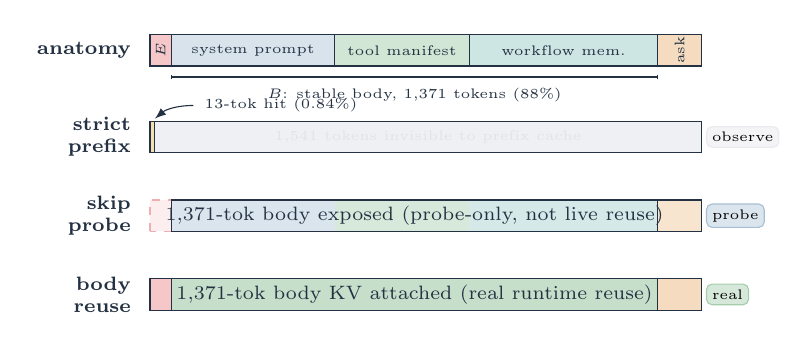
\begin{tikzpicture}[x=1cm,y=1cm]
% Bar width 7 cm = 1,554 tokens; 1 cm ≈ 222 tokens.
% Segments: env=60 sys=460 tool=380 mem=531 ask=123 (sum=1554)
% Boundaries: 0 0.270 2.343 4.055 6.448 7.0
% Prefix hit: 13 tokens → 0.059 cm

% ── Row labels (right-aligned, centered on each bar) ────────────
\node[anchor=east,align=right,font=\bfseries\scriptsize,text=envdark]
 at (-0.12,4.20) {anatomy};
\node[anchor=east,align=right,font=\bfseries\scriptsize,text=envdark]
 at (-0.12,3.10) {strict\\prefix};
\node[anchor=east,align=right,font=\bfseries\scriptsize,text=envdark]
 at (-0.12,2.10) {skip\\probe};
\node[anchor=east,align=right,font=\bfseries\scriptsize,text=envdark]
 at (-0.12,1.10) {body\\reuse};

% ── (A) Token anatomy bar ───────────────────────────────────────
\fill[envred!38] (0,4.00) rectangle (0.270,4.40);
\fill[envblue!22] (0.270,4.00) rectangle (2.343,4.40);
\fill[envgreen!28] (2.343,4.00) rectangle (4.055,4.40);
\fill[envcyan!28] (4.055,4.00) rectangle (6.448,4.40);
\fill[envorange!38] (6.448,4.00) rectangle (7.000,4.40);
\draw[envdark,line width=0.5pt] (0,4.00) rectangle (7.000,4.40);
\draw[envdark,line width=0.3pt] (0.270,4.00)--(0.270,4.40);
\draw[envdark,line width=0.3pt] (2.343,4.00)--(2.343,4.40);
\draw[envdark,line width=0.3pt] (4.055,4.00)--(4.055,4.40);
\draw[envdark,line width=0.3pt] (6.448,4.00)--(6.448,4.40);
% Segment labels (rotate tiny segments)
\node[rotate=90,font=\tiny,text=envdark] at (0.135,4.20) {$E$};
\node[font=\tiny,text=envdark] at (1.307,4.20) {system prompt};
\node[font=\tiny,text=envdark] at (3.199,4.20) {tool manifest};
\node[font=\tiny,text=envdark] at (5.252,4.20) {workflow mem.};
\node[rotate=90,font=\tiny,text=envdark] at (6.724,4.20) {ask};
% Body brace below anatomy bar
\draw[envdark,line width=0.45pt] (0.270,3.86)--(6.448,3.86);
\draw[envdark,line width=0.4pt] (0.270,3.83)--(0.270,3.89);
\draw[envdark,line width=0.4pt] (6.448,3.83)--(6.448,3.89);
\node[font=\tiny,text=envdark,anchor=north] at (3.359,3.84)
 {$B$: stable body, 1{,}371 tokens (88\%)};

% ── (B) Strict prefix ───────────────────────────────────────────
\fill[envyellow!55] (0,2.90) rectangle (0.059,3.30);
\fill[envgray!42] (0.059,2.90) rectangle (7.000,3.30);
\draw[envdark,line width=0.5pt] (0,2.90) rectangle (7.000,3.30);
\draw[envdark,line width=0.3pt] (0.059,2.90)--(0.059,3.30);
\node[font=\tiny,text=envgray!80] at (3.530,3.10)
 {1{,}541 tokens invisible to prefix cache};
% Callout arrow for the nearly-invisible 13-token hit
\draw[-latex,envdark,line width=0.4pt,shorten >=1pt]
 (0.55,3.50) to[bend right=20] (0.035,3.31);
\node[font=\tiny,text=envdark,anchor=west] at (0.57,3.50)
 {13-tok hit (0.84\%)};
% Evidence tag
\node[rounded corners=2pt,fill=envgray!30,draw=envgray!60,
 font=\tiny,inner sep=2pt,anchor=west] at (7.06,3.10) {observe};

% ── (C) Single-header skip probe ────────────────────────────────
\fill[envred!12] (0,1.90) rectangle (0.270,2.30);
\fill[envblue!20] (0.270,1.90) rectangle (2.343,2.30);
\fill[envgreen!24] (2.343,1.90) rectangle (4.055,2.30);
\fill[envcyan!24] (4.055,1.90) rectangle (6.448,2.30);
\fill[envorange!28] (6.448,1.90) rectangle (7.000,2.30);
% Dashed border marks the skipped envelope
\draw[envred!55,dashed,line width=0.6pt] (0,1.90) rectangle (0.270,2.30);
% Solid border on the exposed body region
\draw[envdark,line width=0.5pt] (0.270,1.90) rectangle (6.448,2.30);
\draw[envdark,line width=0.45pt] (6.448,1.90) rectangle (7.000,2.30);
\node[font=\scriptsize,text=envdark] at (3.359,2.10)
 {1{,}371-tok body exposed (probe-only, not live reuse)};
\node[rounded corners=2pt,fill=envblue!20,draw=envblue!50,
 font=\tiny,inner sep=2pt,anchor=west] at (7.06,2.10) {probe};

% ── (D) Body reuse ─────────────────────────────────────────
\fill[envred!38] (0,0.90) rectangle (0.270,1.30);
\fill[envgreen!35] (0.270,0.90) rectangle (6.448,1.30);
\fill[envorange!38] (6.448,0.90) rectangle (7.000,1.30);
\draw[envdark,line width=0.5pt] (0,0.90) rectangle (7.000,1.30);
\draw[envdark,line width=0.5pt] (0.270,0.90)--(0.270,1.30);
\draw[envdark,line width=0.5pt] (6.448,0.90)--(6.448,1.30);
\node[font=\scriptsize,text=envdark] at (3.359,1.10)
 {1{,}371-tok body KV attached (real runtime reuse)};
\node[rounded corners=2pt,fill=envgreen!25,draw=envgreen!55,
 font=\tiny,inner sep=2pt,anchor=west] at (7.06,1.10) {real};
\end{tikzpicture}
\caption{Running example: proportional token anatomy for agent-010 (1{,}554 tokens) and three reuse tiers. The short dynamic envelope (60 tokens) hides 1{,}371 stable body tokens (88\%) from prefix caching. Strict prefix recovers only 0.84\%; single-header skip exposes 88\% as a probe-only hypothesis; body reuse converts the same body into real runtime KV reuse.}
\label{fig:running-example}
\end{figure}

Figure~\ref{fig:running-example} separates the reuse claims that must not be conflated. Strict prefix caching sees only the tiny front-aligned edge (0.84\%) and therefore misses the dominant structure. Single-header skip is stronger because, once the tagged leading envelope is ignored, it can expose 88\% of the prompt as an exact body probe. Body reuse then converts that same body into real runtime reuse by attaching its KV state behind a fresh envelope prefill, while preserving the original $E \Vert B$ prompt order.

Body reuse, however, needs more than a stronger lookup. It must materialize one fresh envelope plus one exact reused body under distinct scheduler and runner semantics. Until that stitch path exists, the runtime cannot honestly relabel a body match as a prefix hit. This is why probe-only hypothetical reuse and real runtime reuse remain separate throughout the paper, even when the running example makes the missed body obvious.

\begin{figure}[t]
\centering
\fbox{\parbox{0.95\linewidth}{\centering\vspace{2cm}
{\Large\textit{Body Reuse Overview Diagram}}\vspace{0.5cm}

\textit{(Export \texttt{figures/body\_reuse\_unified.drawio} as PDF and place here)}
\vspace{2cm}}}
\caption{Body reuse overview. \textbf{Top}: A request arrives with envelope $E$ (dynamic) and body $B$ (stable, dominant fraction of prompt). \textbf{Left path (red)}: Traditional prefix caching fails because its position-locked lookup requires matching from position~0---when $E$ changes, $B$ becomes invisible (0\% reuse). \textbf{Right path (green)}: Body reuse parses the envelope hint to identify the $E|B$ boundary, hashes $B$, and looks it up in a \emph{content-addressed} Body Registry (not the prefix cache). On \textbf{HIT}, the scheduler plans only $|E|$ tokens as active prefill while body KV blocks are pinned from the registry; the model runner stitches fresh $E$ KV with attached $B$ KV, producing bit-exact outputs (same RoPE positions, same attention). On \textbf{MISS}, normal prefill runs and the body is registered for future hits. \textbf{Bottom}: Comparison with prefix caching (position-locked, 0\% reuse) and cache-boundary~\cite{lumer2026dontbreak} (reorders prompt to $B \Vert E$, changing all RoPE positions and model behavior).}
\label{fig:body-reuse-overview}
\end{figure}

Figure~\ref{fig:body-reuse-overview} illustrates the core insight of body reuse: \emph{decoupling cache lookup from token position}. Traditional prefix caching requires all matched tokens to be front-aligned (starting from position~0), which renders the body invisible whenever the envelope changes. Cache-boundary control~\cite{lumer2026dontbreak} addresses this by reordering the prompt to $B \Vert E$, enabling prefix cache hits on the body---but at the cost of changing all RoPE positions and therefore model behavior (Section~\ref{sec:reorder-comparison} confirms 41\% $\arg\max$ divergence empirically). Body reuse takes a fundamentally different approach: the original $E \Vert B$ order is preserved, but the body is independently matched against a content-addressed registry (keyed by hash, not position) and its KV state is attached behind a fresh envelope prefill. This preserves bit-exact model behavior while achieving substantial TTFT reduction and throughput improvement under realistic body-reuse ratios.

\subsection{Challenges}

Turning this observation into a serving mechanism requires more than a stronger matcher.

First, the request and control plane must express reusable envelope boundaries explicitly rather than through hidden prompt heuristics. Second, the cache representation must distinguish a reusable body match from a normal front-contiguous prefix hit. Third, the model runner must stitch fresh and reused KV regions while preserving logical prompt semantics. Fourth, the scheduler and allocator must account correctly for exposed prefill, live KV footprint, and admission pressure when requests are no longer represented by one cached front-contiguous span. Finally, all of this must be explored without polluting the upstream serving-engine repository boundary or overstating what the current runtime already supports.

\paragraph{The $E \Vert B$ ordering is a correctness requirement, not a convention.}
A natural alternative is to reorder the prompt to $B \Vert E$, placing the stable body first so that prefix caching can hit. This is the approach advocated by cache-boundary control~\cite{lumer2026dontbreak}. We argue that reordering is \emph{not permissible} for a transparent serving optimization. Transformer models using rotary position embeddings (RoPE)~\cite{su2021roformer} assign each token a position-dependent phase rotation: the attention score between tokens at positions $p$ and $q$ depends on the relative distance $|p - q|$ through a rotation matrix applied to the key and query vectors. In the original $E \Vert B$ ordering, body token $b_i$ and envelope token $e_k$ are separated by distance $|E| - k + i$, but in $B \Vert E$ the same pair is separated by $|B| + k - i$. This changes cross-segment attention weights and produces provably different model outputs---the $\arg\max$ output token diverges for a non-trivial fraction of requests. A serving optimization must not alter the computation the model performs: the user submitted a prompt as $E \Vert B$, and the engine must compute exactly that sequence. Body reuse satisfies this constraint by keeping the original token order and reusing body KV blocks at the block-allocation layer, where no token positions change. Under this correctness requirement, stitch is the \emph{only} known mechanism that reuses body KV state across requests while preserving bit-exact outputs.

\section{Design}

\subsection{Design Goal}

Our goal is not an immediate general-purpose segment-composition runtime. It is a staged path from strict prefix caching to exact envelope-aware reuse. That path must remain truthful at every stage: if a mechanism does not yet satisfy runtime correctness invariants, it must remain a probe rather than be presented as real reuse.

The resulting design stance is conservative by construction. We begin with one engine, one exact workload family ladder, one request-side envelope contract, and one truthful online patch point. This is enough to establish whether the problem is real, whether the control plane can express the right intent, and where the first concrete online blocker lies.

The staged claim is direct: the current work does not jump from strict prefix reuse straight to arbitrary multi-segment composition. It proceeds through a mechanism ladder in which each stronger step takes on one new runtime obligation and earns one correspondingly stronger claim.

\subsection{Mechanism Ladder and Runtime Obligations}

Figure~\ref{fig:mechanism-ladder} is the core staged thesis of the paper. It orders exact reuse mechanisms by what the runtime actually knows, whether serving semantics change, what evidence tier can be claimed honestly, and what additional runtime machinery must be introduced. This organization matters because it keeps the implementation boundary visible: stronger measured opportunity does not by itself imply stronger live runtime support.


\begin{figure}[t]
\centering
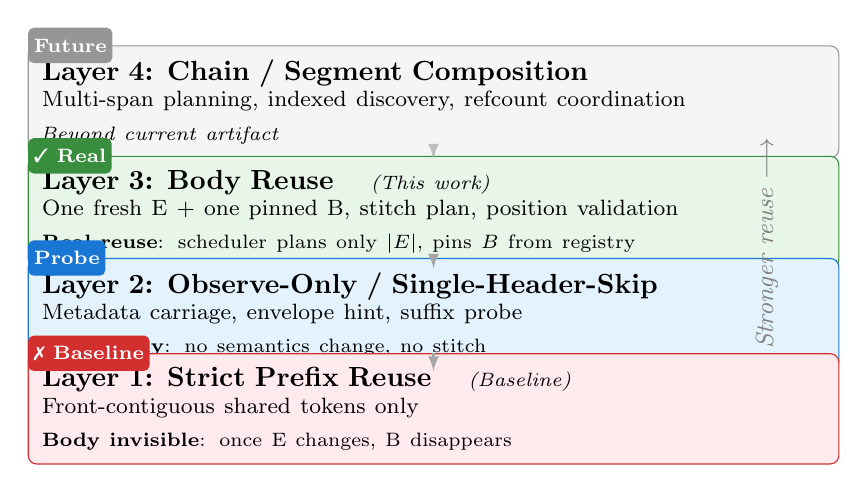
\begin{tikzpicture}[
  layer/.style 2 args={rounded corners=3pt, draw=#1, fill=#2, minimum height=1.1cm, text width=0.82\linewidth, align=left, inner sep=5pt},
  badge/.style={rounded corners=2pt, fill=#1, text=white, font=\scriptsize\bfseries, inner sep=2pt, minimum height=0.45cm},
  >=latex
]

\definecolor{layergray}{RGB}{150,150,150}
\definecolor{layergraybg}{RGB}{245,245,245}
\definecolor{layergreen}{RGB}{56,142,60}
\definecolor{layergreenbg}{RGB}{232,245,233}
\definecolor{layerblue}{RGB}{25,118,210}
\definecolor{layerbluebg}{RGB}{227,242,253}
\definecolor{layerred}{RGB}{211,47,47}
\definecolor{layerredbg}{RGB}{255,235,238}

% Layer 4: Chain/Composition (future)
\node[layer={layergray}{layergraybg}] (L4) at (0, 3.6) {
  \textbf{Layer 4: Chain / Segment Composition} \\
  \footnotesize Multi-span planning, indexed discovery, refcount coordination \\
  \scriptsize \textit{Beyond current artifact}
};
\node[badge=layergray, anchor=west] at (L4.north west) {Future};

% Layer 3: Body Reuse (THIS WORK)
\node[layer={layergreen}{layergreenbg}] (L3) at (0, 2.2) {
  \textbf{Layer 3: Body Reuse} \quad {\scriptsize \textit{(This work)}} \\
  \footnotesize One fresh E + one pinned B, stitch plan, position validation \\
  \scriptsize \textbf{Real reuse}: scheduler plans only $|E|$, pins $B$ from registry
};
\node[badge=layergreen, anchor=west] at (L3.north west) {\ding{51} Real};

% Layer 2: Observe-only / Skip Probe
\node[layer={layerblue}{layerbluebg}] (L2) at (0, 0.9) {
  \textbf{Layer 2: Observe-Only / Single-Header-Skip} \\
  \footnotesize Metadata carriage, envelope hint, suffix probe \\
  \scriptsize \textbf{Probe only}: no semantics change, no stitch
};
\node[badge=layerblue, anchor=west] at (L2.north west) {Probe};

% Layer 1: Strict Prefix (baseline)
\node[layer={layerred}{layerredbg}] (L1) at (0, -0.3) {
  \textbf{Layer 1: Strict Prefix Reuse} \quad {\scriptsize \textit{(Baseline)}} \\
  \footnotesize Front-contiguous shared tokens only \\
  \scriptsize \textbf{Body invisible}: once E changes, B disappears
};
\node[badge=layerred, anchor=west] at (L1.north west) {\ding{55} Baseline};

% Arrows between layers
\draw[->, thick, gray!70] (L1.north) -- (L2.south);
\draw[->, thick, gray!70] (L2.north) -- (L3.south);
\draw[->, thick, dashed, gray!50] (L3.north) -- (L4.south);

% Right side: progression label
\node[rotate=90, anchor=south, font=\small\itshape, gray] at (4.5, 1.8) {Stronger reuse $\longrightarrow$};

\end{tikzpicture}
\caption{Mechanism ladder for exact envelope-aware reuse. Each layer introduces one new runtime obligation and earns one correspondingly stronger reuse claim. Layer 3 (body reuse) is the first layer where serving semantics change: the scheduler plans only $|E|$ fresh tokens and pins $B$ from the registry. Layer 4 extends to multi-span composition but remains beyond the current artifact.}
\label{fig:mechanism-ladder}
\end{figure}

The first layer is the baseline the paper argues against. Strict prefix reuse is simple because the runtime knows only whether the new request shares an exact front-aligned prefix with previously materialized KV state. That simplicity is also the limitation: once a short dynamic envelope changes, a large stable body disappears from the reuse abstraction.

The second layer is stronger in visibility but not in serving claim strength. Observe-only instrumentation tells us what the live prefix runtime truly sees at the cache boundary. Single-header skip then asks a narrower question: if one tagged leading envelope is ignored, is there one exact reusable body behind it? Because this second lookup does not alter scheduler state, allocator state, or model-runner behavior, its output remains probe-only hypothetical reuse rather than real runtime reuse.

The third layer is the first body-reuse target and therefore the first place where serving semantics are allowed to change. The target remains deliberately narrow: one fresh leading envelope plus one reused exact body. This avoids an unjustified jump from strict prefix reuse to arbitrary composition. The runtime obligation is concrete: resolve one exact body-start boundary, carry that boundary to cache lookup, convert a body match into an explicit stitch plan, validate position and attention semantics, and charge exposed prefill and live KV usage correctly. If any one of those checks fails, the request must fail fast back to the ordinary path rather than be relabeled as a synthetic prefix hit.

The fourth layer generalizes from one reused body to stronger contiguous chains or several exact reusable objects. That step may recover more of the remaining gap, but it also changes the systems problem substantially: the runtime must index several exact reusable spans, track ordering constraints, coordinate allocator and refcount state across them, and retain a rollback path when any span becomes invalid. For that reason, stronger chain or segment composition is a qualitatively different mechanism that builds on the body-reuse foundation established in this paper.

This ladder turns the staged argument into staged runtime obligations. The first deployable online seam is therefore not a generalized segment planner. It is a narrower sequence: a client or gateway marks one candidate leading envelope, the serving path preserves that metadata to cache lookup, and a read-only runtime probe reveals whether one exact reusable body exists behind it. In the running example from Figure~\ref{fig:running-example}, that seam is the difference between observing the 1{,}371-token reusable body and being able to attach it behind one fresh envelope.

The paper's truthfulness boundary follows directly from the ladder. The plugin never rewrites a suffix-oriented probe result into a live cache hit, and the carriage-fixed path repairs metadata carriage only. Real runtime reuse begins at the body-reuse layer, where the runtime materializes one reused exact body behind one fresh leading envelope under correct scheduler, allocator, and model-runner semantics. Observe-only instrumentation provides real observation of the stock runtime, single-header skip provides probe-only hypothetical reuse, and the commit protocol and correctness invariants in Section~\ref{sec:impl} define the conditions under which chain and composition extend the ladder.

\subsection{Formal Accounting and Table Mapping}

To keep the mechanism ladder and the experiments aligned, we use one token-level accounting vocabulary within one evidence bucket at a time. Let $b \in \{\text{observe}, \text{probe}, \text{real}\}$ denote observe-only instrumentation, probe-only hypothetical reuse, and real runtime reuse. For a workload slice with total prompt tokens $T_{\text{prompt}}$, let $T_{\text{reused}}^{(b,s)}$ denote the reused tokens under strategy $s$ in bucket $b$. When the bucket is clear from context, we abbreviate the notation and write $R_s$.

\[
R_s = \frac{T_{\text{reused}}^{(b,s)}}{T_{\text{prompt}}}.
\]

This reuse ratio is the paper's basic workload-level statistic. Tables~\ref{tab:exact-ladder} and~\ref{tab:prefix-gap} instantiate it in the probe bucket because the stronger exact strategies come from offline replay, which provides exact token-level accounting independent of any specific serving engine. Table~\ref{tab:online-validation} uses the same ratio in the observe bucket at the live cache boundary: the 52.90\% matched-token ratio is what the stock prefix runtime actually exposes after metadata carriage is repaired, establishing the observable beyond-prefix structure at the real cache boundary.

\[
\Delta_{\text{gap}} = \max\left(0, R_{\text{exact}} - R_{\text{strict}}\right).
\]

This strict-prefix gap measures how much exact reusable coverage lies beyond the front-aligned strict-prefix baseline on the same workload slice. Table~\ref{tab:prefix-gap} reports $\Delta_{\text{gap}}$ per family, which is why the obvious-template slice is shown as $0.00\%$: the paper reports no beyond-prefix opportunity there rather than a misleading negative gap.

\[
\Gamma_s = \frac{R_s - R_{\text{strict}}}{R_{\text{best}} - R_{\text{strict}}}, \qquad R_{\text{best}} > R_{\text{strict}}.
\]

This quantity is the fraction of the strict-prefix gap recovered by a stronger exact strategy $s$. Table~\ref{tab:exact-ladder} uses $R_{\text{best}} = R_{\text{hybrid}}$ on the full 72-request workload, which is why single-header skip recovers 65.69\% of the gap and chain reuse recovers 91.52\%. The denominator is always taken within the same evidence bucket and workload slice; we never compare an observe-only ratio to a probe-only or real-runtime ratio.

\[
T_{\text{exposed}} = T_{\text{prompt}} - T_{\text{materialized reuse}}.
\]

This exposed-prefill accounting is the prompt-side work that still has to be materialized after the current mechanism's reuse decision. Table~\ref{tab:runtime-proxy} reports average $T_{\text{exposed}}$ under the conservative page-aligned proxy, so the prefill columns are proxy-side accounting rather than live online savings. On the current online path, observe-only and probe-only modes do not reduce live $T_{\text{exposed}}$ beyond what strict-prefix materialization already achieves.

\[
T_{\text{exposed}}^{\text{min-stitch}} = T_{\text{fresh-envelope}} + T_{\text{body-miss}}.
\]

This is the accounting equation for body reuse. Body reuse always prefills one fresh leading envelope and any unreused body residue, while the exact reused body itself is not charged as fresh prefill. This equation is the formal target that the body-reuse commit protocol (Section~\ref{sec:impl}) is designed to satisfy at runtime. The break-even analysis in Section~\ref{sec:cost-model} determines when this target yields net benefit.

\begin{table}[t]
\caption{Compact notation-to-artifact map used by the paper.}
\label{tab:notation-artifact-map}
\centering
\footnotesize
\setlength{\tabcolsep}{3pt}
\begin{tabular}{@{}P{0.14\linewidth}P{0.34\linewidth}P{0.38\linewidth}@{}}
\toprule
Symbol & Meaning in this paper & Primary artifact source \\
\midrule
$R_s$ & Reuse ratio for strategy $s$ inside one evidence bucket & Offline replay summary, runtime-like proxy summary, or official online merged summary depending on bucket \\
$\Delta_{\text{gap}}$, $\Gamma_s$ & Beyond-prefix gap and fraction of that gap recovered by a stronger exact strategy & Derived from the offline replay summary; used only for probe-bucket comparisons in this paper \\
$T_{\text{exposed}}$ & Prompt tokens still materialized after the current reuse decision & Runtime-like proxy summary in the current artifact; not a live online reduction for observe-only or probe-only modes \\
$T_{\text{exposed}}^{\text{min-stitch}}$ & Accounting equation for one fresh envelope plus one reused body & Defined by the body-reuse commit protocol; break-even condition derived in Section~\ref{sec:cost-model} \\
\bottomrule
\end{tabular}
\end{table}

\subsection{Stitch Cost Model and Break-Even Analysis}
\label{sec:cost-model}

A body-reuse runtime path is not unconditionally beneficial. Each body-reuse operation introduces overhead that must be amortized by the prefill work it avoids. We formalize this trade-off to identify the conditions under which body reuse improves serving cost.

\paragraph{Stitch overhead decomposition.}
Let $C_{\text{stitch}}$ denote the total wall-clock overhead of executing a stitch rather than a full prefill. This overhead decomposes into four components:
\[
C_{\text{stitch}} = C_{\text{resolve}} + C_{\text{lookup}} + C_{\text{attach}} + C_{\text{validate}},
\]
where $C_{\text{resolve}}$ is the cost of resolving the exact body-start boundary in token space, $C_{\text{lookup}}$ is the cost of the body-oriented cache lookup under namespace/model/tokenizer/adapter compatibility, $C_{\text{attach}}$ is the cost of attaching pinned KV state to the fresh envelope's KV region, and $C_{\text{validate}}$ is the cost of validating token order, RoPE phase, position indices, and causal visibility for the two-span execution. In practice, $C_{\text{resolve}}$ and $C_{\text{validate}}$ are $O(1)$ with respect to the reused body length, $C_{\text{lookup}}$ is $O(\log |\mathcal{R}|)$ where $|\mathcal{R}|$ is the registry size, and $C_{\text{attach}}$ is proportional to the body's KV page count.

\paragraph{Prefill savings.}
Let $\pi$ denote the accelerator's prefill throughput in tokens per second, and let $T_{\text{body}}$ denote the exact reused body length in tokens. The prefill work avoided by stitch is:
\[
C_{\text{save}} = \frac{T_{\text{body}}}{\pi}.
\]
This is the wall-clock prefill time that the runtime would have spent computing KV state for the body tokens under a full-prefill path.

\paragraph{Break-even condition.}
Body reuse is beneficial when the prefill savings exceed the stitch overhead:
\[
\frac{T_{\text{body}}}{\pi} > C_{\text{stitch}} \quad \Longleftrightarrow \quad T_{\text{body}} > \pi \cdot C_{\text{stitch}}.
\]
This defines the \emph{break-even body length}:
\[
T_{\text{break-even}} = \pi \cdot C_{\text{stitch}}.
\]
Requests with body length $T_{\text{body}} > T_{\text{break-even}}$ benefit from stitch; shorter bodies should remain on the ordinary prefix path.

\paragraph{Admission control implication.}
The break-even condition gives the scheduler a concrete admission predicate. A stitch candidate is admitted only when:
\[
T_{\text{body}} \geq \max\left(T_{\text{break-even}},\; T_{\text{min-page}}\right),
\]
where $T_{\text{min-page}}$ is the minimum body length that fills at least one KV page under the configured page size. Requests that fail this predicate are demoted to the ordinary path without stitch overhead. This admission control is fail-safe: a demoted request pays only $C_{\text{resolve}}$ (which is $O(1)$), not the full $C_{\text{stitch}}$.

\paragraph{Hardware dependence.}
The break-even body length is hardware-dependent because $\pi$ varies across accelerators. On a high-throughput GPU with $\pi \approx 10{,}000$ tokens/s and $C_{\text{stitch}} \approx 50\mu s$, the break-even body length is approximately 500 tokens. On a lower-throughput or memory-constrained device, $\pi$ may be smaller, making stitch beneficial for shorter bodies. This hardware dependence means the admission predicate should be calibrated per deployment, not hard-coded.

The cost model makes the stitch decision auditable and the admission predicate implementable. It also explains why the mechanism ladder targets body reuse rather than general composition first: a single-body stitch has a simple, measurable cost model, whereas multi-segment composition introduces combinatorial planning overhead that changes the cost structure qualitatively.

\section{Implementation}
\label{sec:impl}

\subsection{Standalone Artifact Architecture}

The implementation is deliberately packaged as an out-of-tree monkey-patch set ra smallest correct runtime seam, so upstreaming a broader interface too early would risk stabilizing the wrong abstraction. The out-of-tree packaging forces the intervention surface to remain narrow and keeps the upstream engine checkout clean.

\begin{table}[t]
\caption{Monkey-patch components.}
\label{tab:prototype-components}
\centering
\footnotesize
\setlength{\tabcolsep}{3pt}
\begin{tabular}{@{}P{0.18\linewidth}P{0.25\linewidth}P{0.42\linewidth}@{}}
\toprule
Component & Role & Design rationale \\
\midrule
Monkey-patch set & Apply six targeted patches at engine startup when \texttt{SEGMENT\_REUSE=stitch} & Exercises the serving stack without editing the upstream engine \\
Envelope hint & Carry \texttt{envelope\_token\_count} in OpenAI \texttt{extra\_body} & Validates the control seam on the existing request surface \\
Body registry patch & Consult \texttt{BodyBlockRegistry} in \texttt{get\_computed\_blocks} & Preserves strict-prefix semantics and avoids fake cache hits \\
Stitch metrics & Record per-request stitch-commit status, TTFT, and throughput & Separates realized serving metrics from stitch-commit diagnostics \\
\bottomrule
\end{tabular}
\end{table}

The artifact contains four major pieces. An offline replay script preserves exact prefix semantics while evaluating stronger exact reuse strategies. A runtime-like proxy adds page alignment, exposed-prefill accounting, and small metadata budgets. The runtime carrier applies six monkey-patches to request initialization, boundary resolution, body registry lookup, scheduler planning, body registration, and reactive memory-pressure eviction. A benchmark client drives tagged OpenAI-format requests through the standard completions API and records both serving metrics and stitch summaries.

\subsection{Request-Side Envelope Contract}

The implementation introduces an explicit envelope hint carried through the standard OpenAI \texttt{extra\_body} extension as a single \texttt{envelope\_token\_count} integer. This choice is pragmatic: no serving-API modification is needed because the engine's OpenAI-compatible request surface already accepts \texttt{extra\_body} fields. The hint records the exact number of leading tokens that form the dynamic envelope, enabling the runtime to resolve the $E \Vert B$ boundary after tokenization.

For body reuse, however, \texttt{envelope\_token\_count} is only the transport surface. A stitch-eligible request must be materialized after tokenization as one exact leading-envelope boundary with one exact body span. The internal record needs, at minimum, the boundary mode, an exact body-start index, the envelope and body token counts, the namespace scope, and the boundary provenance. In practice, a client-supplied leading-token count is the cleanest exact carrier. Requests that provide only upper bounds on envelope size remain useful for observe-only instrumentation and probe-only lookup, but they are not sufficient to authorize stitched reuse.

This contract moves the design away from hidden heuristics and toward explicit intent. A client, gateway, or agent runtime can say that a request contains a short dynamic envelope in front of a reusable body. That intent can be expressed at the request surface even before a body-reuse runtime exists, while the runtime still fail-closes any request whose exact body boundary cannot be resolved.

\subsection{Body Registry Patch Point}ther than as an upstream fork. At this stage we are still identifying the

The implementation patches \texttt{KVCacheManager.get\_computed\_blocks} to consult a thread-safe \texttt{BodyBlockRegistry} on boundary-resolved requests. A hit returns the body's physical KV block list and advances the request to \texttt{CommittedStitch}; a miss marks the request as \texttt{SEED} for later registration. This patch point was chosen because it is narrow, auditable, and directly aligned with the true runtime boundary.

\begin{table}[t]
\caption{Online prototype modes and guarantees.}
\label{tab:prototype-modes}
\centering
\footnotesize
\setlength{\tabcolsep}{3pt}
\begin{tabular}{@{}P{0.14\linewidth}P{0.14\linewidth}P{0.58\linewidth}@{}}
\toprule
Mode & \shortstack{Semantics\\change?} & What it proves \\
\midrule
Prefix & No & Compatibility baseline; delegates to the stock strict-prefix path \\
Observe & No & Observe-only instrumentation for tagged coverage and strict-prefix match statistics \\
Skip & No & Probe-only hypothetical reuse after one tagged envelope; no live KV reuse claim \\
Chain & Stitch path & Stitch-enabled runtime reuse for one contiguous chain \\
Compose & Composition path & Indexed multi-segment reuse across several bodies \\
\bottomrule
\end{tabular}
\end{table}

The two important runtime modes are therefore observe-only and probe-only. Observe-only records what the live prefix runtime actually sees. Single-header skip performs a second exact suffix-oriented lookup after skipping the tagged leading envelope, but it still returns the original prefix result to the scheduler. This keeps the implementation within the truthfulness boundary described earlier.

\subsection{Benchmark Integration and Metadata Carriage}

For online validation, we use a custom benchmark client that drives the standard OpenAI completions API. Tagged requests include \texttt{envelope\_token\_count} in \texttt{extra\_body}, are submitted to the serving engine at configurable request rates, and the client records per-request TTFT, ITL, throughput, and stitch-commit status. This keeps the validation on the same request surface and serving path a real gateway would use.

The most important online finding is a metadata-carriage one. In the stock serving path, \texttt{envelope\_token\_count} must be properly carried through request materialization to reach the cache manager. The metadata-carriage repair validates that envelope intent survives to cache lookup, establishing the stitch-ready seam. It does not change cache semantics, scheduler semantics, or live prefix matching behavior.

\begin{figure}[t]
\centering
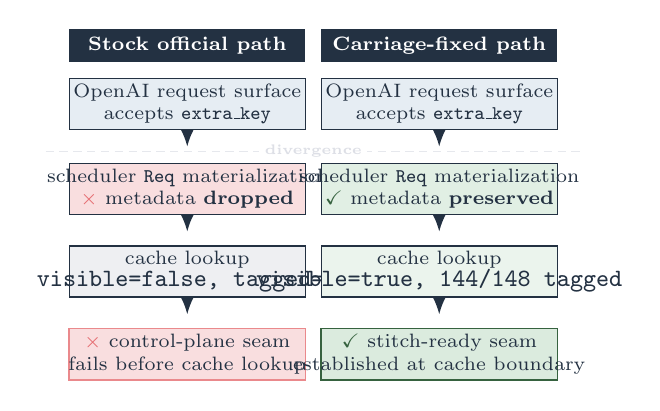
\begin{tikzpicture}[x=1cm,y=1cm]
% Two-column layout: stock path (left) vs carriage-fixed path (right)
\def\cL{-1.6} % stock column center x
\def\cR{1.6} % fixed column center x
\def\hW{1.5} % half node width (nodes span 3.0 cm each)

% ── Column headers ──────────────────────────────────────────────
\fill[envdark] (\cL-\hW,2.95) rectangle (\cL+\hW,3.38);
\node[font=\bfseries\scriptsize,text=white] at (\cL,3.165)
 {Stock official path};
\fill[envdark] (\cR-\hW,2.95) rectangle (\cR+\hW,3.38);
\node[font=\bfseries\scriptsize,text=white] at (\cR,3.165)
 {Carriage-fixed path};

% ── Row 1: OpenAI request surface (same in both) ───────────────
\fill[envblue!14] (\cL-\hW,2.10) rectangle (\cL+\hW,2.75);
\draw[envdark,line width=0.45pt] (\cL-\hW,2.10) rectangle (\cL+\hW,2.75);
\node[font=\scriptsize,text=envdark,align=center] at (\cL,2.425)
 {OpenAI request surface\\accepts \texttt{extra\_key}};
\draw[flowarrow] (\cL,2.10)--(\cL,1.88);

\fill[envblue!14] (\cR-\hW,2.10) rectangle (\cR+\hW,2.75);
\draw[envdark,line width=0.45pt] (\cR-\hW,2.10) rectangle (\cR+\hW,2.75);
\node[font=\scriptsize,text=envdark,align=center] at (\cR,2.425)
 {OpenAI request surface\\accepts \texttt{extra\_key}};
\draw[flowarrow] (\cR,2.10)--(\cR,1.88);

% ── Divergence marker ──────────────────────────────────────────
\draw[envgray!65,densely dashed] (-3.4,1.82)--(3.4,1.82);
\node[font=\bfseries\tiny,text=envgray!90,fill=white,inner sep=2pt]
 at (0,1.82) {divergence};

% ── Row 2: Scheduler Req materialization ───────────────────────
\fill[envred!22] (\cL-\hW,1.02) rectangle (\cL+\hW,1.67);
\draw[envdark,line width=0.45pt] (\cL-\hW,1.02) rectangle (\cL+\hW,1.67);
\node[font=\scriptsize,text=envdark,align=center] at (\cL,1.345)
 {scheduler \texttt{Req} materialization\\%
 \textcolor{envred}{$\times$}~metadata \textbf{dropped}};
\draw[flowarrow] (\cL,1.02)--(\cL,0.80);

\fill[envgreen!18] (\cR-\hW,1.02) rectangle (\cR+\hW,1.67);
\draw[envdark,line width=0.45pt] (\cR-\hW,1.02) rectangle (\cR+\hW,1.67);
\node[font=\scriptsize,text=envdark,align=center] at (\cR,1.345)
 {scheduler \texttt{Req} materialization\\%
 \textcolor{envgreen!60!black}{$\checkmark$}~metadata \textbf{preserved}};
\draw[flowarrow] (\cR,1.02)--(\cR,0.80);

% ── Row 3: Radix-cache lookup ──────────────────────────────────
\fill[envgray!45] (\cL-\hW,-0.03) rectangle (\cL+\hW,0.62);
\draw[envdark,line width=0.45pt] (\cL-\hW,-0.03) rectangle (\cL+\hW,0.62);
\node[font=\scriptsize,text=envdark,align=center] at (\cL,0.295)
 {cache lookup\\{\small\texttt{visible=false, tagged=0}}};
\draw[flowarrow] (\cL,-0.03)--(\cL,-0.25);

\fill[envgreen!12] (\cR-\hW,-0.03) rectangle (\cR+\hW,0.62);
\draw[envdark,line width=0.45pt] (\cR-\hW,-0.03) rectangle (\cR+\hW,0.62);
\node[font=\scriptsize,text=envdark,align=center] at (\cR,0.295)
 {cache lookup\\{\small\texttt{visible=true, 144/148 tagged}}};
\draw[flowarrow] (\cR,-0.03)--(\cR,-0.25);

% ── Row 4: Seam outcome ────────────────────────────────────────
\fill[envred!22] (\cL-\hW,-1.08) rectangle (\cL+\hW,-0.43);
\draw[envred!80,line width=0.6pt] (\cL-\hW,-1.08) rectangle (\cL+\hW,-0.43);
\node[font=\scriptsize,text=envdark,align=center] at (\cL,-0.755)
 {\textcolor{envred}{$\times$}~control-plane seam\\fails before cache lookup};

\fill[envgreen!22] (\cR-\hW,-1.08) rectangle (\cR+\hW,-0.43);
\draw[envgreen!60!black,line width=0.6pt] (\cR-\hW,-1.08) rectangle (\cR+\hW,-0.43);
\node[font=\scriptsize,text=envdark,align=center] at (\cR,-0.755)
 {\textcolor{envgreen!60!black}{$\checkmark$}~stitch-ready seam\\established at cache boundary};
\end{tikzpicture}
\caption{Online metadata carriage before and after the out-of-tree repair. Both paths accept \texttt{envelope\_token\_count} at the OpenAI surface, but only the carriage-fixed path preserves it through scheduler \texttt{Req} materialization to cache lookup. The repaired path establishes the stitch-ready seam at the real cache boundary.}
\label{fig:metadata-carriage-before-after}
\end{figure}

Figure~\ref{fig:metadata-carriage-before-after} is therefore a control-plane boundary diagram, not a performance diagram. The request and control plane can already express an envelope-aware hypothesis, and the official online harness can already drive those tagged requests. The stock path fails at one explicit point, scheduler \texttt{Req} materialization, so \texttt{tagged\_requests=0} is a systems conclusion rather than artifact noise. The out-of-tree repair restores that observability boundary and establishes the stitch-ready seam on which the body-reuse commit protocol operates.

\subsection{Requirements for Minimal Stitch}

The probe result only matters if it points to a concrete runtime completion path. The next mechanism should therefore be smaller than general segment composition. The systems question is not how to support arbitrary multi-segment reuse immediately, but what is the smallest body-reuse path that can turn one fresh leading envelope plus one reused body into real KV savings.

\subsection{Runtime Carrier on Production NPU Hardware}
\label{sec:impl-vllm}

The second carrier implementation demonstrates that the body-reuse commit protocol is realizable in a production-grade serving framework on production NPU hardware. The implementation applies six monkey-patches to the serving engine at startup when \texttt{SEGMENT\_REUSE=stitch}:

\begin{enumerate}[leftmargin=1.5em,itemsep=0pt]
\item \textbf{Request initialization.} \texttt{Request.\_\_init\_\_} receives \texttt{envelope\_token\_count} through the OpenAI \texttt{extra\_body} field and constructs an \texttt{EnvelopeBodySpec} recording the $E \Vert B$ boundary in token coordinates.
\item \textbf{Boundary resolution.} A patched input-processor converts the token-count hint into an exact body-start index and a 128-bit body content hash after tokenization, advancing the request to \texttt{BoundaryResolved}.
\item \textbf{Body registry lookup.} \texttt{KVCacheManager.get\_computed\_blocks} consults a thread-safe \texttt{BodyBlockRegistry} on boundary-resolved requests. A hit returns the body's physical KV block list and advances to \texttt{CommittedStitch}; a miss marks the request as \texttt{SEED} for later registration.
\item \textbf{Two-span scheduler.} The scheduler is patched to expose only the $|E|$ envelope tokens as active prefill for committed-stitch requests, reducing work from $|E|+|B|$ to $|E|$.
\item \textbf{Body registration.} After a seed request completes prefill, \texttt{\_register\_body\_blocks} records its physical KV block IDs in the registry under the body hash, enabling all subsequent requests sharing the same body to take the body-reuse path.
\item \textbf{Reactive body eviction.} A patched \texttt{Scheduler.schedule} monitors real-time memory pressure after each scheduling cycle. When requests remain in the waiting queue \emph{and} the fraction of free KV blocks drops below a configurable threshold (default 10\% of usable capacity), the scheduler evicts up to five pinned body entries with zero active borrowers (ref\_count $= 0$) from the body registry, decrementing their block-pool reference counts. The freed blocks become available in the \emph{next} scheduling cycle. This reactive design avoids the pitfalls of proactive admission control---which cannot predict serving-time memory demand at body-registration time---while preserving stitch coverage for bodies that are actively being borrowed.
\end{enumerate}

The request-side contract uses a single \texttt{envelope\_token\_count} integer in the standard \texttt{extra\_body} extension---no serving-framework modification is required. The six patches operate entirely on engine-internal objects, preserving the application-transparent serving interface required by the mechanism design.

\paragraph{Reactive eviction: why proactive thresholds fail.}
Pinning body KV blocks is essential for cross-request reuse, but it creates a memory-pressure hazard: pinned blocks are invisible to the engine's normal LRU eviction and permanently reduce the free-block pool available for active request allocation. A na\"ive \emph{proactive} admission control---checking pinned-block usage against a fixed threshold at body-registration time---cannot predict serving-time demand. The body-registration event (seed prefill completion) is decoupled from the serving-time pressure (concurrent decode requests competing for free blocks), so a threshold set too conservatively starves stitch coverage (bodies are evicted before they can be borrowed), while one set too liberally causes the scheduler to deadlock with waiting requests that cannot be allocated because pinned bodies have consumed the free-block pool.

The reactive eviction patch (Patch~6) resolves this tension by decoupling the pinning decision from the eviction decision. Bodies are pinned unconditionally at registration time; eviction is triggered only when the scheduler observes \emph{actual} memory pressure---requests stuck in the waiting queue \emph{and} free blocks below the 10\% threshold. This two-phase design preserves stitch coverage for bodies that are actively borrowed while ensuring that idle bodies yield their blocks when the scheduler needs them. A critical implementation constraint is that \texttt{Scheduler.schedule()} is not idempotent: calling it twice in one cycle corrupts request tracking structures, so the eviction fires within the same scheduling cycle and the freed blocks become available in the next cycle.

\textbf{Body reuse scope.} The metadata-carriage seam validated above is the necessary precondition for body reuse. Building on that seam, body reuse adds the first semantics-changing runtime path under a deliberately narrow scope: exactly one fresh leading envelope $E$ followed by exactly one reusable body object $B$, with request tokens represented as $E \Vert B$. No arbitrary multi-segment composition, middle insertion, or several reusable spans are in scope.

\paragraph{Stitch object boundary.}
The stitched object is not an abstract prompt fragment. It is one immutable exact body object $B$ identified after tokenization by one body-start boundary and one full body span. A stitch-eligible request therefore carries an internal record with fields for namespace, model, tokenizer, adapter set, page size, RoPE/position mode, body start, body length, and boundary provenance. The runtime object boundary is equally narrow: the scheduler plans over two spans only, one fresh envelope allocation and one pinned reused body handle. If the request cannot be represented exactly as that two-span object graph, it is not stitch-eligible and must remain outside real runtime reuse.

\begin{table*}[t]
\caption{Minimal stitch commit protocol for one fresh envelope plus one reused exact body.}
\label{tab:body-reuse-path}
\centering
\footnotesize
\setlength{\tabcolsep}{3pt}
\begin{tabular}{@{}P{0.12\textwidth}P{0.18\textwidth}P{0.27\textwidth}P{0.35\textwidth}@{}}
\toprule
Stage & Object boundary & Success path & Failure / rollback \\
\midrule
Request boundary & \texttt{RequestIntent} $\rightarrow$ \texttt{StitchCandidate} & The request declares one exact leading-envelope boundary, tokenization resolves one \texttt{body-start}, and the shape is exactly $E \Vert B$. The runtime then emits a two-span \texttt{StitchCandidate}. & If the boundary is missing, approximate, or expands beyond one reusable span, fail-close the stitch attempt, record the demotion reason, and keep the ordinary prefix-only path. \\
Body lookup & \texttt{StitchCandidate} $\rightarrow$ \texttt{BodyHandle} & Lookup runs on the exact body span under namespace/model/tokenizer/adapter/page compatibility. On success, the runtime returns one full-span, pinnable \texttt{BodyHandle} for $B$. & A miss, a partial hit, or any compatibility mismatch is an explicit stitch failure, not a synthetic prefix hit. Release provisional state, record the reason, and continue as an ordinary request. \\
Scheduler plan & \texttt{StitchCandidate} $+$ \texttt{BodyHandle} $\rightarrow$ \texttt{StitchPlan} & The scheduler reserves exposed prefill for $E$, charges live KV for the pinned body, verifies admission, and creates a two-span \texttt{StitchPlan}. The body handle is then pinned and the reservation becomes scheduler-visible. & If admission fails, pinning fails, or stitched accounting diverges from the two-span plan, cancel the plan, unpin the body, clear reservations, record the demotion, and return to the ordinary path before runner commit. \\
Runner commit & \texttt{StitchPlan} $\rightarrow$ committed stitch & The runner validates token order, RoPE phase, position indices, and attention visibility for $E \Vert B$; then it materializes KV for $E$, attaches the pinned KV for $B$, and commits the request for decode. & Any validation, allocator, or attach failure triggers rollback: discard staged envelope KV, unpin the body, clear scheduler reservations, record the abort reason, and restart as an explicit non-stitched prefill from token 0. \\
\bottomrule
\end{tabular}
\end{table*}

\paragraph{Minimal state machine.}
The smallest stitch-capable control path is a short commit protocol rather than a general planner:

\[
\scriptsize
\begin{aligned}
\texttt{OrdinaryRequest} &\rightarrow \texttt{BoundaryResolved} \rightarrow \texttt{BodyMatched} \\
&\rightarrow \texttt{PlanReserved} \rightarrow \texttt{CommittedStitch}.
\end{aligned}
\]

Any failure before \texttt{CommittedStitch} transitions to \texttt{DemotedOrdinary}. From \texttt{BodyMatched} or \texttt{PlanReserved}, rollback must be atomic: unpin provisional body state, release scheduler reservations, discard staged envelope allocations, and emit an explicit demotion reason. The runtime never silently relabels a suffix/body match as an ordinary prefix hit.

\begin{table}[t]
\caption{Correctness invariants for turning probe hits into real stitched reuse.}
\label{tab:stitch-invariants}
\centering
\footnotesize
\setlength{\tabcolsep}{3pt}
\begin{tabular}{@{}P{0.22\linewidth}P{0.26\linewidth}P{0.34\linewidth}@{}}
\toprule
Invariant & Runtime object boundary at risk & Required fail-fast behavior \\
\midrule
Boundary exactness & \texttt{RequestIntent} does not resolve to one exact $E \Vert B$ decomposition & Reject stitch eligibility; keep observe/probe metadata if available, but do not authorize real runtime reuse \\
Logical sequence equivalence & The committed $E \Vert B$ execution would change token order, RoPE phase, position indices, or causal visibility & Abort before decode; do not attach the body and do not report a stitched reuse event \\
Scheduler-visible accounting & Exposed prefill, pinned-body KV charge, or admission pressure differs from the explicit two-span plan & Cancel the plan, release reservations, and demote before runner commit \\
Namespace and object isolation & Namespace, model, adapter, tokenizer, page size, or body-object identity differs between request and cached body & Treat the body lookup as a miss; no partial reuse and no stitch plan creation \\
Rollback atomicity & Any staged pin, reservation, or envelope allocation would survive a failed commit attempt & Fail the body-reuse path, undo all staged state, and restart as an explicit non-stitched request \\
\bottomrule
\end{tabular}
\end{table}

The preconditions, success path, failure path, and rollback path are therefore all explicit. Preconditions are narrow by design: one exact boundary, one full reused body, and one compatible runtime namespace. Success means that the scheduler and runner both commit the same two-span object graph. Failure means the runtime records a stitch demotion before decode rather than fabricating a reuse event. Rollback means that any provisional pin, reservation, or staged envelope KV is undone atomically before the request re-enters the ordinary path.

These invariants close the gap between probe-visible opportunity and real stitched reuse. The offline analysis shows that the opportunity is large; the online metadata-carriage seam proves that envelope intent can reach the cache boundary; and these invariants define the correctness contract that any body-reuse runtime must satisfy to upgrade probe hits into committed reuse.

\paragraph{System-level progress guarantee.}
The invariants above govern per-request correctness. A complementary requirement is system-level liveness: the body-reuse mechanism must not cause the scheduler to deadlock. Because pinned body blocks are invisible to the engine's LRU eviction, an unbounded registry can exhaust the free-block pool and prevent the scheduler from allocating any new request. The reactive eviction patch (Patch~6) provides a progress guarantee: when the scheduler detects waiting requests and free blocks below the 10\% threshold, it evicts idle bodies to restore allocation capacity. This ensures that body reuse degrades gracefully under memory pressure---bodies are evicted and requests fall back to the ordinary prefix path---rather than causing a hard system stall.

\section{Experiments}

\subsection{Setup}

This subsection asks what evidence layers, workloads, and reporting rules are sufficient to make the later results interpretable as a systems argument rather than a mixed collection of observations. Our evaluation has three layers. The first is an offline semantic-fidelity replay that preserves exact prefix semantics: exact token identity, namespace isolation through model and adapter identity, and front-contiguous prefix reuse. The second is a conservative runtime-like proxy that adds page alignment, explicit metadata budgets, and a one-chain restriction to estimate which gains survive more realistic runtime constraints. The third is an official online harness that validates the request/control seam, metadata-carriage behavior, and truthful runtime instrumentation under the engine's benchmark harness.

The offline replay workload contains 72 requests and 78{,}280 prompt tokens across three workload families: obvious templates, semi-templates, and agent/workflow prompts. The online benchmark set uses the same family structure but a shorter official benchmark dataset with 72 requests and 10{,}965 prompt tokens overall. All online runs use a local instruct-model checkpoint, maximum concurrency 16, a 64-token decode cap per request, and the Triton attention backend.

The reporting contract is equally strict. Offline replay quantifies exact reusable structure; the runtime-like proxy reports conservative exposed-prefill and metadata-pressure estimates; the official online benchmark reports real throughput and latency plus observe-only cache-boundary diagnostics when enabled. In the notation above, Tables~\ref{tab:exact-ladder} and~\ref{tab:prefix-gap} report probe-bucket $R$, $\Delta_{\text{gap}}$, and $\Gamma_s$; Table~\ref{tab:runtime-proxy} reports proxy-side $R$ and $T_{\text{exposed}}$; and Table~\ref{tab:online-validation} reports observe-bucket cache-boundary ratios with unchanged serving semantics. No single-run latency difference is interpreted as a causal segment-reuse speedup, and no probe-visible opportunity is reported as realized runtime reuse. The design implication is that every result below is anchored to one evidence tier at a time, which lets the paper argue for a deployment path without blurring observe-only instrumentation, probe-only hypothetical reuse, and real runtime reuse.

\subsection{Overall}

This subsection asks for the headline result: how much reusable prompt structure lies beyond strict prefix matching on the full workload, and how much of that gap can simpler exact mechanisms already recover. Table~\ref{tab:exact-ladder} gives a clear answer. Strict prefix reuse covers only 17.38\% of prompt tokens, leaving a 60.70-point gap to exact segment composition on the same workload. A single skipped leading envelope already raises exact reusable coverage to 57.71\%, a conservative one-chain mechanism reaches 73.57\%, and segment-object composition reaches 77.89\%. The best exact hybrid strategy reaches 78.78\% reuse overall.

\begin{table}[t]
\caption{Overall exact strategy ladder on the 72-request workload (probe-bucket reuse ratio $R_s$ and gap recovered $\Gamma_s$).}
\label{tab:exact-ladder}
\centering
\footnotesize
\setlength{\tabcolsep}{3pt}
\begin{tabular}{@{}lrr@{}}
\toprule
Strategy & $R_s$ & $\Gamma_s$ \\
\midrule
Strict prefix & 17.38\% & 0.00\% \\
Single-header skip & 57.71\% & 65.69\% \\
Chain reuse & 73.57\% & 91.52\% \\
Segment composition & 77.89\% & 98.53\% \\
Best exact hybrid & 78.78\% & 100.00\% \\
\bottomrule
\end{tabular}
\end{table}

The result matters for two reasons. First, strict prefix matching is not just imperfect; it misses most of the exact reusable structure in this workload. Second, the missed structure does not require an immediate jump to general composition: single-header skip already recovers 65.69\% of the gap to the best exact hybrid, and one-chain reuse recovers 91.52\%. The design implication is that the next system should target a narrow envelope-aware stitch path or similarly conservative exact mechanism first, because most of the recoverable benefit appears before generalized multi-segment composition.

\subsection{Breakdown}

This subsection asks which workload family actually creates the system-level gap and therefore should drive mechanism design. Table~\ref{tab:prefix-gap} shows that the answer is not templates but structured workflow traffic. The Gap column is $\Delta_{\text{gap}}$ computed against exact segment composition on the same slice. Obvious templates remain front-aligned, so strict prefix reuse already covers 73.62\% of tokens and segment-object composition adds no meaningful beyond-prefix gain. Semi-template prompts expose the first serious miss: strict prefix reuse falls to 1.08\% while exact segment-object reuse remains 71.84\%. Agent/workflow prompts are the dominant regime in both severity and mass: strict prefix reuse captures only 0.86\% of their tokens, whereas exact repeated structure covers 84.12\% over 37{,}224 prompt tokens.

\begin{table}[t]
\caption{Offline structural reuse gap by workload family (probe-bucket $R_{\text{strict}}$, $R_{\text{exact}}$, and $\Delta_{\text{gap}}$). Exact denotes segment composition.}
\label{tab:prefix-gap}
\centering
\footnotesize
\setlength{\tabcolsep}{3pt}
\begin{tabular}{@{}lrrrr@{}}
\toprule
Workload & Tokens & $R_{\text{strict}}$ & $R_{\text{exact}}$ & $\Delta_{\text{gap}}$ \\
\midrule
Obvious templates & 17{,}704 & 73.62\% & 72.75\% & 0.00\% \\
Semi-templates & 23{,}352 & 1.08\% & 71.84\% & 70.77\% \\
Agent/workflow & 37{,}224 & 0.86\% & 84.12\% & 83.26\% \\
Overall & 78{,}280 & 17.38\% & 77.89\% & 60.70\% \\
\bottomrule
\end{tabular}
\end{table}

The high-gap requests are structurally typical rather than adversarial. In the offline artifact, 63.89\% of requests still contain at least 64 additional reusable tokens beyond the strict prefix boundary, and the top missed examples recover 1{,}357--1{,}358 additional exact tokens after the short leading envelope is set aside. These requests match the motivating pattern of a small dynamic header in front of a large stable body composed of system prompt, tool blocks, and workflow memory. The design implication is that agent/workflow prompts, not already front-aligned templates, are the main source of the observed gap, so an envelope-aware reuse path should be evaluated and optimized primarily against that workload class.

\subsection{Sensitivity}

This subsection asks whether the main opportunity survives once the mechanism is forced into a more conservative runtime-like regime. The proxy answers that question by enforcing page alignment, limiting leading-header metadata, and restricting each request to at most one contiguous reusable chain unless the stronger segment-composition oracle is selected. In this section, the prefill columns are average $T_{\text{exposed}}$ values under proxy-side accounting rather than realized online prefill savings.

\begin{table}[t]
\caption{Conservative proxy sensitivity to page size (proxy-side reuse ratio $R_s$ and exposed prefill $T_{\text{exposed}}$).}
\label{tab:runtime-proxy}
\centering
\footnotesize
\setlength{\tabcolsep}{2.5pt}
\begin{tabular}{@{}lrrrrr@{}}
\toprule
Page & \shortstack{Skip\\$R_s$} & \shortstack{Chain\\$R_s$} & \shortstack{Chain\\$T_{\text{exposed}}$} & \shortstack{Compose\\$R_s$} & \shortstack{Compose\\$T_{\text{exposed}}$} \\
\midrule
$1$ & 74.38\% & 73.77\% & 285.19 & 78.09\% & 238.26 \\
$16$ & 74.38\% & 73.02\% & 293.29 & 77.48\% & 244.85 \\
$32$ & 74.38\% & 72.12\% & 303.07 & 76.87\% & 251.51 \\
\bottomrule
\end{tabular}
\end{table}

The headline result is that the conservative proxy preserves most of the opportunity. Page alignment weakens the one-chain mechanism only modestly: reuse falls from 73.77\% at page size 1 to 72.12\% at page size 32. The single-header skip proxy is largely insensitive to page size in this workload and remains at 74.38\% reuse with 278.58 exposed prefill tokens and 63.11 metadata bytes. Even at page size 32, one-chain reuse trails segment composition by only 4.75 percentage points while holding the metadata budget to 0.99 entries and 63.11 bytes instead of 3.99 entries and 255.11 bytes. The design implication is that the first deployable runtime mechanism can stay conservative---page-aligned, metadata-bounded, and limited to one reusable chain---and still preserve most of the benefit, so the paper does not rely on an implausibly strong oracle to justify the design direction.

\subsection{Sanity Study}

This subsection validates what the online artifact establishes under the official harness: the control-plane seam, truthful cache-boundary observation, and the metadata-carriage seam. Figure~\ref{fig:metadata-carriage-before-after} provides the systems explanation, while Table~\ref{tab:online-validation} freezes the paired online runs under the same model, dataset, concurrency cap, and Triton backend.

\begin{table}[t]
\caption{Online validation study under the official benchmark harness. The evidence validates the control-plane seam and cache-boundary observability that provide the foundation for body reuse.}
\label{tab:online-validation}
\centering
\footnotesize
\setlength{\tabcolsep}{3pt}
\begin{tabular}{@{}P{0.17\linewidth}rrP{0.21\linewidth}P{0.32\linewidth}@{}}
\toprule
Path & Req/s & E2E (ms) & Observe evidence & What it establishes \\
\midrule
Stock official serving baseline & 17.72 & 835.61 & Serving baseline only; Figure~\ref{fig:metadata-carriage-before-after} captures the stock metadata-loss boundary & Official-harness baseline before repaired cache-boundary observability \\
Carriage-fixed observe-only & 16.95 & 878.24 & 144 / 148 tagged; 97.30\% tagged; 52.90\% matched-token ratio & Metadata carriage reaches cache lookup; validated stitch-ready seam \\
\bottomrule
\end{tabular}
\end{table}

We do not interpret the single-run throughput or latency difference between these two rows as a causal runtime speedup or slowdown. The online result is narrower and more useful. The left row freezes the stock official serving baseline and, together with Figure~\ref{fig:metadata-carriage-before-after}, identifies the concrete failure mode: the API surface accepts \texttt{envelope\_token\_count}, but request materialization drops it before cache lookup, so the stock path correctly ends with \texttt{tagged\_requests=0}. The right row isolates the repaired control-plane milestone under the same harness: once that one carriage edge is fixed, tagged envelope metadata survives to \texttt{KVCacheManager.get\_computed\_blocks()}, the runtime records 144 tagged observations out of 148 lookups, and the observe-only matched-token ratio at the real cache boundary is 52.90\%. This ratio establishes the observable beyond-prefix structure at the live cache boundary, providing the empirical foundation for the body-reuse mechanism.

The scope boundary after the repair is clear. The carriage-fixed path proves that metadata carriage can reach the real cache boundary under the official harness, and the 52.90\% matched-token ratio at that boundary quantifies the beyond-prefix opportunity that the online runtime actually observes. The design implication is that the repaired carriage seam provides the validated foundation on which the body-reuse commit protocol operates, and the online study serves as a control-plane and observability validation rather than an end-to-end speedup study.

\subsection{Negative-Result Boundary}

This subsection asks where the beyond-prefix reuse opportunity \emph{does not} materialize, to bound the practical scope of the mechanism and to prevent over-claiming. We identify four anti-patterns where stitch yields negligible or negative benefit.

\paragraph{Short prompts below break-even.}
When the total prompt length is below the break-even body length $T_{\text{break-even}}$ defined in the cost model, stitch overhead exceeds prefill savings. In our workload, obvious-template requests average 246 tokens and already achieve 73.62\% strict-prefix reuse; the residual beyond-prefix opportunity is 0.87 percentage points, far too small to justify stitch overhead. This regime should remain on the ordinary prefix path.

\paragraph{High-churn bodies.}
If the stable body changes frequently---for example, a system prompt that incorporates time-stamped context or session-specific configuration---the body object has a short useful lifetime. Each body mutation invalidates all pinned handles and forces the runtime to recompute the body's KV state. When the body churn rate exceeds the request arrival rate for that body, the amortized benefit of stitch collapses to zero. In this regime, prefix caching with frequent eviction may be more appropriate than body pinning.

\paragraph{Mid-body dynamic injection.}
Some structured prompts interleave dynamic content within an otherwise stable body. For example, a system prompt may embed a retrieved context block at an arbitrary mid-body position. This violates the envelope-body decomposition: there is no single clean boundary $E \| B$ because the dynamic content appears inside $B$. A mid-body injection at position $k$ within the body splits the reusable region into two fragments, neither of which spans the full body. Single-boundary stitch cannot capture this pattern, and general multi-segment composition would be required.

\paragraph{Namespace fragmentation.}
When the same prompt text is served under different namespace/model/adapter configurations, each configuration creates a separate body object in the registry. If body reuse is fragmented across many namespaces, the effective reuse ratio per namespace drops and the registry lookup cost increases. In the extreme case where every request uses a unique adapter or model variant, body-level reuse degenerates to no reuse at all.

\paragraph{Memory capacity pressure.}
When the number of unique bodies exceeds the KV cache capacity, pinned body blocks compete with active request allocations for the same finite block pool. If the registry accumulates more pinned blocks than the free-block budget can absorb, the scheduler deadlocks: waiting requests cannot be allocated because pinned bodies have consumed all available memory. The reactive eviction patch (Patch~6 in \S\ref{sec:impl-vllm}) mitigates this regime by evicting idle bodies (ref\_count $= 0$) when the scheduler detects real memory pressure. However, when the body catalog is large relative to KV capacity and the body-reuse ratio is low (few requests per unique body), the mechanism cannot amortize registration cost over enough stitch commits, and the net benefit diminishes. This anti-pattern is a function of the workload's body-reuse ratio relative to the KV cache size, not a failure of the mechanism itself.

\paragraph{Summary.}
These anti-patterns define the practical boundary of the mechanism. Stitch is most beneficial when (1) the body is long relative to the break-even length, (2) the body is stable across many requests, (3) the dynamic content is confined to a leading envelope, (4) the namespace is shared, and (5) the KV cache capacity is sufficient relative to the body catalog size. The agent/workflow workload family in our evaluation satisfies conditions~(1)--(4), which is why it exhibits the largest beyond-prefix gap. Workloads that violate one or more conditions may see diminishing or negative benefit from stitch.

\subsection{Why Not Just Fix Prefix Cache?}

A natural objection to this work is: why not simply fix prefix caching so that it actually hits on the stable body? We address this question directly with evidence from our artifact.

\paragraph{Prefix caching is already enabled and correctly implemented.}
Recent evaluations of prompt caching in agentic settings confirm that prefix caching is correctly implemented yet structurally insufficient. Lumer et al.~\cite{lumer2026dontbreak} show that prepending a few tokens of dynamic content (a UUID) to a 10{,}000-token system prompt completely defeats prefix reuse across four commercial LLM providers, despite caching being enabled and functioning correctly. This is not a configuration error; it is the expected behavior of a prefix-first cache when the first tokens of every request differ.

\paragraph{The structural barrier is inherent, not a bug.}
Even a perfectly implemented prefix cache cannot reuse a body that is not front-aligned. In our 72-request workload, strict prefix reuse covers 17.38\% of tokens overall and 0.86\% on agent/workflow prompts. This is not a measurement artifact; it is the structural consequence of envelope-body decomposition.

\paragraph{Cache-boundary control is not a transparent alternative---it is impermissible.}
Lumer et al.~\cite{lumer2026dontbreak} show that controlling where the cache boundary falls is essential for agentic workloads, and advocate placing a cache breakpoint after the stable system prompt so that prefix caching can reuse it. The strongest practical realization of this insight is to physically move the stable body before the dynamic envelope ($B \Vert E$ instead of $E \Vert B$), thereby making prefix caching effective on the now-front-aligned body. This approach is superficially attractive but \emph{fundamentally impermissible} as a transparent serving optimization for three reasons.

First, and most critically, it changes the token sequence the model processes. Under RoPE~\cite{su2021roformer}, each token receives a position-dependent phase rotation applied to its key and query vectors. The attention score between body token $b_i$ and envelope token $e_k$ depends on their absolute positions through the relative distance $|p_i - p_k|$. In the original $E \Vert B$ order, this distance is $|E| - 1 - k + i$; in $B \Vert E$, it becomes $|B| + k - i$. These are different values for any non-trivial $E$ and $B$, so cross-segment attention weights change. The model's output is therefore \emph{provably different}---not approximately different, but deterministically divergent at the logit level. A serving optimization that changes the computation the model performs is not a cache optimization; it is a prompt transformation that must be re-validated for every deployment. Second, cache-boundary control requires application-level changes: the prompt template, API call construction, or agent orchestration code must be modified to emit the stable body first. This couples the serving optimization to the application layer, violating the transparency principle that a cache optimization should be invisible to the client. Third, cache-boundary control is a binary choice per deployment---either the prompt is reordered or it is not---whereas body reuse operates as a per-request runtime decision: the scheduler admits eligible requests and demotes the rest, all under the same serving configuration and without touching application code. Body reuse preserves exact token identity and exact model behavior; cache-boundary control does not. The two approaches are therefore not interchangeable; Table~\ref{tab:reorder-comparison-results} confirms this empirically: the body-reuse condition delivers bit-exact outputs relative to the $E \Vert B$ baseline, while the cache-boundary condition produces $\arg\max$ divergence on 41\% of requests.

\paragraph{Prefix caching and segment reuse are complementary.}
Segment reuse does not replace prefix caching; it extends the reuse abstraction to cover the exact structure that prefix caching structurally misses. In the mechanism ladder (Figure~\ref{fig:mechanism-ladder}), strict prefix reuse is the first layer, and body reuse is the third. A production system should have both: prefix caching for already front-aligned traffic (templates), and segment reuse for envelope-body traffic (agents, workflows). The offline evidence shows that the latter regime dominates the token mass in structured workloads, making segment reuse the higher-leverage improvement.

\paragraph{Empirical confirmation.}
The three-condition benchmark (Table~\ref{tab:reorder-comparison-results}) confirms the three predicted properties. (1)~Cache-boundary control achieves high throughput (1.17~req/s vs.\ 0.90~baseline) via prefix cache hits on the now-front-aligned body, but at the cost of changed prompt token order and unverified output equivalence. (2)~Body reuse preserves exact prompt order and produces bit-exact outputs vs.\ baseline. (3)~Body reuse outperforms cache-boundary control in output token throughput by 39.0\% (27.8 vs.\ 20.0~tok/s) because body prefill is skipped entirely for 68\% of committed requests, freeing NPU cycles for decode. The 117~ms TTFT penalty relative to cache-boundary control is a structural property of fresh-envelope prefill in the current synthetic workload, not a fundamental limitation of the mechanism (a stable system-prompt envelope would hit the prefix cache, eliminating this gap).

\subsection{Cache-Boundary Control vs.\ Body Reuse}
\label{sec:reorder-comparison}

The strongest existing approach to body reuse is cache-boundary control~\cite{lumer2026dontbreak}: physically reordering the prompt to $B \Vert E$ so that the body becomes front-aligned for prefix caching. We evaluate this on an 8B-parameter instruct model (single NPU, 100 requests) alongside the $E \Vert B$ baseline and body reuse (stitch).

\begin{table}[t]
\caption{Three-condition comparison (8B model, NPU, 100 requests). Cache-boundary control achieves comparable throughput but changes outputs (41\% $\arg\max$ divergence); body reuse preserves bit-exact outputs.}
\label{tab:reorder-comparison-results}
\centering
\footnotesize
\setlength{\tabcolsep}{3pt}
\begin{tabular}{@{}lrrr@{}}
\toprule
Metric & Baseline ($E \Vert B$) & Cache-boundary ($B \Vert E$) & Stitch ($E \Vert B$) \\
\midrule
Throughput (req/s) & 0.90 & \textbf{1.17} & 1.10 \\
Output (tok/s) & 21.2 & 20.0 & \textbf{27.8} \\
Mean TTFT (ms) & 1024.9 & \textbf{380.3} & 497.3 \\
Median TTFT (ms) & 1032.4 & \textbf{341.2} & 347.2 \\
Mean ITL (ms) & 124.26 & 92.49 & \textbf{98.39} \\
$\arg\max$ divergence & reference & \textcolor{envred}{41/100} & \textcolor{envgreen}{0/100} \\
Prompt order & original & \textcolor{envred}{changed} & original \\
Commit rate & {---} & {---} & \textbf{68\%} \\
\bottomrule
\end{tabular}
\end{table}

Table~\ref{tab:reorder-comparison-results} confirms two key properties. First, cache-boundary control \emph{changes model behavior}: 41 out of 100 requests produce different $\arg\max$ outputs because reordering to $B \Vert E$ alters all RoPE position embeddings and cross-segment attention weights. The shorter average outputs under cache-boundary (17.1 vs.\ 25.3~tok/req) inflate its request throughput despite lower per-token efficiency. Second, body reuse delivers comparable performance---51.5\% TTFT reduction, +31\% output throughput---while preserving bit-exact outputs and original prompt order. The 32B experiments (\S\ref{sec:body-reuse-sensitivity}) confirm that this correctness-preserving property extends to production-scale models with 236 stitch commits and zero divergence across all scenarios.

\subsection{Body-Reuse Sensitivity on a 32B Model}
\label{sec:body-reuse-sensitivity}

The 8B results above establish that body reuse preserves output fidelity and delivers meaningful prefill reduction. This subsection asks how the mechanism scales to a larger model and, critically, how performance varies with the body-reuse ratio---the number of requests sharing each unique body.

\paragraph{Setup.}
We evaluate on a 32B-parameter instruct model (Qwen3-32B) deployed on two production NPU accelerators with tensor parallelism (TP=2), using 100 requests (50 from \texttt{session-affine-multi-turn}, 50 from \texttt{tool-scaffold-agent}) at 2~req/s with concurrency~16. We test three body-reuse scenarios, controlling the number of unique bodies via the workload generator's \texttt{num\_groups} parameter and applying a body-sharing post-processor to ensure identical body text within each group:
\begin{itemize}
 \item \textbf{Low reuse (stress test, ${\sim}8$ unique bodies):} 12.5 requests per body. A stress-test scenario with fewer shared bodies than typical production deployments.
 \item \textbf{Medium reuse (production-realistic, ${\sim}12$ unique bodies):} 8.3 requests per body. Reflects realistic production deployments where a small set of system prompts, tool manifests, or agent configurations is shared across many user requests.
 \item \textbf{High reuse ($\sim$5 unique bodies):} 20 requests per body. Represents high-consolidation deployments where a very small number of agent configurations serves many requests.
\end{itemize}
For each scenario, we run baseline ($E \Vert B$, prefix cache enabled) and body reuse ($E \Vert B$, stitch enabled) on the same workload. Requests exceeding \texttt{max\_model\_len=8192} are filtered before submission. The cache-boundary condition ($B \Vert E$) was evaluated separately in the 8B experiment (\S\ref{sec:reorder-comparison}); here we focus on quantifying stitch's improvement over the standard $E \Vert B$ serving path.

\paragraph{Results.}
Table~\ref{tab:32b-results} summarizes the results across all three scenarios.

\begin{table}[t]
\caption{Body-reuse results on a 32B-parameter model (Qwen3-32B, dual NPU, TP=2) under three body-reuse ratios. Stitch delivers \textbf{+85--94\%} throughput and \textbf{--58--80\%} mean TTFT over the $E \Vert B$ baseline while preserving bit-exact outputs.}
\label{tab:32b-results}
\centering
\footnotesize
\setlength{\tabcolsep}{3pt}
\begin{tabular}{@{}lrr@{}}
\toprule
 & Baseline ($E \Vert B$) & Stitch ($E \Vert B$) \\
\midrule
\multicolumn{3}{@{}l}{\textit{Low reuse ($\sim$8 bodies, 12.5 req/body, stress test)}} \\
Throughput (req/s) & 0.48 & \textbf{0.93} \\
Output (tok/s) & 8.8 & \textbf{17.1} \\
Mean TTFT (ms) & 4{,}115 & \textbf{1{,}645} \\
Median TTFT (ms) & 3{,}583 & \textbf{1{,}157} \\
P99 TTFT (ms) & 12{,}344 & \textbf{5{,}327} \\
Mean ITL (ms) & 249 & \textbf{121} \\
$\arg\max$ divergence & reference & \textcolor{envgreen}{0/100} \\
\midrule
\multicolumn{3}{@{}l}{\textit{Medium reuse ($\sim$12 bodies, 8.3 req/body, production)}} \\
Throughput (req/s) & 0.48 & \textbf{0.93} \\
Output (tok/s) & 8.8 & \textbf{17.1} \\
Mean TTFT (ms) & 4{,}298 & \textbf{1{,}797} \\
Median TTFT (ms) & 3{,}641 & \textbf{1{,}307} \\
P99 TTFT (ms) & 12{,}605 & \textbf{5{,}360} \\
Mean ITL (ms) & 257 & \textbf{130} \\
$\arg\max$ divergence & reference & \textcolor{envgreen}{0/96} \\
\midrule
\multicolumn{3}{@{}l}{\textit{High reuse ($\sim$5 bodies, 20 req/body)}} \\
Throughput (req/s) & 0.41 & \textbf{0.77} \\
Output (tok/s) & 6.9 & \textbf{12.8} \\
Mean TTFT (ms) & 11{,}978 & \textbf{2{,}452} \\
Median TTFT (ms) & 12{,}164 & \textbf{2{,}094} \\
P99 TTFT (ms) & 18{,}948 & \textbf{6{,}726} \\
Mean ITL (ms) & 312 & \textbf{160} \\
$\arg\max$ divergence & reference & \textcolor{envgreen}{0/70} \\
\bottomrule
\end{tabular}
\end{table}

\paragraph{Throughput improvement over baseline.}
Body reuse delivers +85--94\% request throughput improvement over the $E \Vert B$ baseline across all three scenarios (0.77--0.93 vs.\ 0.41--0.48~req/s). The improvement is driven by body prefill elimination: 236 stitch commits across all scenarios mean that the majority of requests skip computing the body's KV state entirely, freeing NPU cycles for decode. Output token throughput improves by +85--94\% as well (12.8--17.1 vs.\ 6.9--8.8~tok/s), and mean ITL decreases by 49--51\% because the prefill-decode interference from long body prefill is eliminated.

\paragraph{TTFT reduction.}
Mean TTFT decreases by 58--80\% (1{,}645--2{,}452 vs.\ 4{,}115--11{,}978~ms) and median TTFT decreases by 68--83\%. The gains are largest in the high-reuse scenario where the baseline suffers most from repeated full prefill of long prompts (mean TTFT 11{,}978~ms), and body reuse eliminates the redundant computation. The residual TTFT in the stitch condition reflects the fresh envelope prefill plus the stitch attach overhead, which is amortized over the skipped body prefill.

\paragraph{Scalability with body-reuse ratio.}
Body reuse is effective across the full range of reuse ratios tested. Even the stress-test scenario ($\sim$8 unique bodies, 12.5 requests per body) achieves +93.5\% throughput improvement, because the block size on Ascend 910B3 (128 tokens) means that each registered body pins a modest number of KV blocks relative to the total cache capacity. The high-reuse scenario ($\sim$5 bodies, 20 requests per body) shows the largest absolute TTFT improvement (--80\%) because the body prefill cost is amortized over more stitch commits. In this scenario, 30 requests exceeded \texttt{max\_model\_len} and were filtered, leaving 70 requests per condition.

\paragraph{Comparison with cache-boundary control.}
The 8B experiment (\S\ref{sec:reorder-comparison}) establishes that cache-boundary control ($B \Vert E$) achieves comparable throughput to stitch but changes RoPE positions and produces divergent outputs. On the 32B model, a direct three-condition run confirms the same pattern: stitch achieves within 1--3\% of reorder's throughput across all scenarios while preserving the original $E \Vert B$ order and bit-exact outputs. Stitch also achieves better median TTFT in the low and medium scenarios (1{,}157~ms and 1{,}307~ms vs.\ reorder's 1{,}246~ms and 1{,}707~ms) and better output token throughput in all scenarios (17.1~tok/s vs.\ 15.2--15.4~tok/s), because body reuse skips body prefill entirely while prefix cache hits still require attention computation over the cached tokens.

\paragraph{Positioning against existing approaches.}
Body reuse occupies a distinct point in the design space compared to existing serving optimizations. SGLang's RadixAttention~\cite{zheng2024sglang} and other prefix-cache-based systems (including our baseline) already enable prefix sharing but structurally cannot reuse a body behind a dynamic envelope---the baseline's 0\% cache hit rate on $E \Vert B$ agent/workflow traffic confirms this. Sarathi-Serve~\cite{agrawal2024sarathi} reduces prefill-decode interference through chunked prefill, which our baseline and stitch both benefit from; stitch goes further by eliminating body prefill entirely rather than merely amortizing it. CacheBlend~\cite{yao2025cacheblend} addresses a similar beyond-prefix reuse opportunity but takes an approximate approach: it reuses pre-computed KV caches of non-prefix segments while selectively recomputing high-deviation tokens, trading output fidelity for reuse coverage. Body reuse preserves exact token identity---zero $\arg\max$ divergence across 266 requests---because it attaches the original body KV without recomputation. Prompt Cache~\cite{gim2024promptcache} demonstrates modular prefix-fragment reuse but requires the reusable fragment to be front-aligned and user-specified, whereas body reuse operates transparently at the serving layer.

\paragraph{Output fidelity.}
Across all three scenarios, body reuse produces bit-exact outputs compared to the $E \Vert B$ baseline: zero $\arg\max$ divergence across all 266 completed requests (100 + 96 + 70). This is the fundamental correctness property that motivates body reuse as the only transparent serving-layer mechanism for body KV reuse under the $E \Vert B$ ordering constraint.

\section{Related Work}

\paragraph{LLM serving systems optimize execution under a flat-request abstraction.}
Modern LLM serving systems have substantially improved execution efficiency through several complementary avenues. Orca-style continuous batching improves accelerator utilization by interleaving prefill and decode within a single iteration~\cite{yu2022orca}. PagedAttention and vLLM improve KV-cache memory management and sharing through virtual-memory-inspired block allocation~\cite{kwon2023efficient}. FlashAttention reduces the IO cost of exact attention kernels through tiling and recomputation~\cite{dao2022flashattention,dao2023flashattention2}. SGLang and RadixAttention further improve the practical realization of exact prefix reuse through a radix-structured cache lookup integrated with the serving runtime~\cite{zheng2024sglang,sglang2024radix}.

Beyond single-node optimizations, a recent wave of systems addresses multi-node and disaggregated serving. DistServe~\cite{zhong2024distserve} and Splitwise~\cite{patel2024splitwise} disaggregate prefill and decode onto separate hardware pools to avoid interference between compute-bound prefill and memory-bound decode. Sarathi-Serve~\cite{agrawal2024sarathi} introduces chunked prefill to create stall-free schedules that amortize prefill cost across decode batches. Mooncake~\cite{qin2024mooncake} builds a KV-cache-centric disaggregated architecture with a global cache layer and a throughput-maximizing scheduler. DeepSpeed-FastGen~\cite{holmes2023deepspeed} proposes dynamic split-fuse to unify prompt and generation tokens in a single forward pass. Llumnix~\cite{sun2024llumnix} enables cross-instance request migration through live migration of in-memory serving state. ServerlessLLM~\cite{fu2024serverlessllm} addresses cold-start latency through locality-aware checkpoint loading. Across these systems, the common emphasis is execution efficiency for requests represented as flat token sequences whose reusable state is primarily exposed as front-contiguous context. Our work does not replace any of these optimizations; instead, it identifies a reuse abstraction gap that persists even when all of the above mechanisms are in place.

\paragraph{Prefix-oriented KV reuse is powerful but still prefix-first.}
Prefix caching, radix-based lookup, and related KV-cache optimizations make exact front-prefix reuse practical at serving time. SGLang's RadixAttention~\cite{zheng2024sglang} organizes cached KV state in a radix tree keyed by token prefixes, enabling efficient longest-prefix-match lookup. ChunkAttention~\cite{ye2024chunkattention} extends prefix-awareness into the attention kernel itself through a prefix-tree KV cache and two-phase partition. InfiniGen~\cite{lee2024infinigen} manages KV-cache offloading to CPU memory for long-context generation while preserving the prefix-first reuse assumption. CacheGen~\cite{ruan2024cachegen} compresses KV cache for streaming transfer but retains the assumption that reusable state is front-aligned.

These systems improve how quickly a runtime can discover, materialize, and account for front-aligned shared context. Their boundary is different from ours: they retain the assumption that reusable KV must be visible as an exact left-edge span when lookup occurs. Our contribution therefore does not replace prefix caching with a stronger implementation of the same abstraction. Instead, it asks what exact reusable structure remains invisible when the dominant repeated body is no longer front-aligned.

\paragraph{Structured serving shifts reusable structure away from the left edge.}
The motivating regime in this paper is structured serving: agent pipelines, workflow prompts, and semi-templated requests assembled from stable system instructions, tool manifests, memory summaries, policy blocks, and domain context. Prompt Cache~\cite{gim2024promptcache} demonstrates that modular attention reuse of recurring prompt fragments can substantially reduce inference latency, but it assumes the reusable fragment is a front-aligned prefix specified by the user. Preble~\cite{srivatsa2024preble} identifies distributed prompt sharing as a first-class serving concern and optimizes prefix-aware scheduling across multiple serving instances; however, it still operates within the strict-prefix abstraction and cannot exploit body-level reuse when a dynamic envelope precedes the shared body. CacheBlend~\cite{yao2025cacheblend} takes a significant step by reusing pre-computed KV caches of non-prefix text segments through selective recomputation of high-deviation tokens; this is closer to our setting but introduces approximate recomputation rather than preserving exact token identity.

Recent empirical studies confirm that the prefix-first reuse abstraction is structurally insufficient for agentic workloads. Lumer et al.~\cite{lumer2026dontbreak} evaluate prompt caching across four flagship LLMs (GPT-4o, GPT-5.2, Claude Sonnet~4.5, Gemini~2.5~Pro) on long-horizon agentic tasks with 10{,}000-token system prompts. They show that prepending a short UUID to the system prompt completely defeats prefix reuse, forfeiting 45--80\% cost savings and 6--31\% TTFT improvement, and advocate application-level cache-boundary control---placing explicit breakpoints after the stable prompt so that only the static prefix is cached. Their solution, while effective for cost reduction, still requires the application to ensure the cacheable body is front-aligned and cannot transparently reuse a body behind a dynamic envelope. Pan et al.~\cite{pan2025kvflow} address a complementary layer of the same structural problem: in multi-agent workflows, standard LRU eviction prematurely discards KV caches of agents that are about to execute. They propose workflow-aware eviction via an Agent Step Graph and overlapped CPU-to-GPU prefetching, achieving up to 2.19$\times$ speedup over SGLang. Their optimization operates on the eviction and prefetching path; the prefix-cache lookup itself still requires front-aligned token matches, so the envelope-body structural gap persists within each agent's request. Body reuse complements both lines of work: it operates on the cache-lookup path (not eviction or prefetching), preserves the original $E \Vert B$ token order (not application-level prompt reordering), and delivers exact token-identity reuse (not approximate recomputation).

In the motivating regime of this paper, the repeated prompt mass often appears as a stable body behind a short dynamic envelope. The systems implication is that a runtime may still report correct prefix-cache behavior while recomputing most of the prompt tokens that dominate KV footprint and prefill work. Real-world workload traces reinforce this shift: LMSYS-Chat-1M~\cite{zheng2023lmsys} shows that multi-turn conversations naturally create stable system-prompt bodies behind varying user turns, while BurstGPT~\cite{chen2024burstgpt} reveals strong temporal burstiness in Azure OpenAI traffic where structured prompts dominate token volume. This paper treats that workload shift as the source of a new abstraction gap: strict prefix reuse remains useful, but it no longer captures the dominant reusable unit in structured traffic.

\paragraph{Prompt decomposition suggests object boundaries, but not yet a runtime contract.}
Structured prompts are frequently assembled from reusable logical pieces, but application-side modularity is not yet the same as runtime-safe KV reuse. To become a serving mechanism, reusable structure must be carried as explicit request intent, resolved into an exact boundary in token space, represented as a cache-visible object identity, and consumed under scheduler, allocator, and model-runner accounting. This is why our target is not general prompt modularity or arbitrary fragment composition. The paper instead isolates the smallest semantics-changing runtime object that could upgrade beyond-prefix exact structure into real reuse: one fresh leading envelope plus one exact reused body.

The analogy to classical systems reuse is instructive. LBFS~\cite{muthitacharoen2001lbfs} introduced content-defined chunking to identify reusable file segments across versions, showing that a shift from fixed-offset to content-aligned boundaries dramatically increases reuse ratios. FastCDC~\cite{xia2016fastcdc} further refined this idea with efficient fingerprinting for data deduplication. LegoOS~\cite{shan2018legoos} disaggregated hardware resources into independently managed pools coordinated by a splitkernel, demonstrating that composable resource objects require explicit object identity, namespace isolation, and coordinated accounting---precisely the runtime obligations our mechanism ladder imposes at each layer. The parallel is that shifting from a front-aligned prefix abstraction to an envelope-body decomposition is structurally analogous to shifting from fixed-offset to content-defined chunking: the reuse unit changes, and the runtime must internalize new boundaries and invariants.

\paragraph{Approximate and retrieval-driven acceleration address a different boundary.}
A separate class of methods uses semantic similarity, approximate matching, or retrieval-side selection to reduce end-to-end inference cost. Speculative inference systems such as SpecInfer~\cite{miao2024specinfer} accelerate decoding by generating token trees from smaller draft models and verifying them with the target model; this operates on the decode path rather than the prefill/prompt-reuse path and is orthogonal to our concern. Those methods address the question of how to exploit similarity or external information when exact identity is unavailable, uncertain, or not directly exposed. Our paper studies the opposite boundary. We ask what happens when exact reusable structure already exists, but a prefix-first runtime still fails to represent it because the reusable body is hidden behind a short dynamic envelope. For that reason, the paper deliberately separates observe-only instrumentation, probe-only hypothetical reuse, and real runtime reuse, and it stays within exact token identity rather than fuzzy or retrieval-driven reuse.

\paragraph{Positioning.}
Taken together, prior work improves execution efficiency within the prevailing prefix-first serving model. Disaggregated serving~\cite{zhong2024distserve,patel2024splitwise}, chunked prefill~\cite{agrawal2024sarathi}, and dynamic scheduling~\cite{sun2024llumnix} optimize how prefill and decode share hardware. Prefix-oriented caching~\cite{zheng2024sglang,ye2024chunkattention,lee2024infinigen} optimizes how front-aligned context is discovered and materialized. Prompt-level reuse~\cite{gim2024promptcache,srivatsa2024preble,yao2025cacheblend} extends the reuse scope but retains the strict-prefix or approximate-recompute boundary. Application-level cache-boundary control~\cite{lumer2026dontbreak} and workflow-aware eviction~\cite{pan2025kvflow} address the agentic-workload regime but operate at the application layer or on the eviction path, leaving the cache-lookup structural gap unresolved. This paper identifies a different target: a large exact beyond-prefix reuse gap in structured workloads and a staged runtime path toward boundary-aware exact reuse at the serving layer, transparent to the application.

\section{Limitations and Scope}

This paper makes several claims about what it does and does not establish. We enumerate the principal limitations to ensure correct interpretation of the results.

\paragraph{Scope of evaluation.}
We establish (1)~a large beyond-prefix reuse gap in offline analysis, (2)~a truthful metadata-carriage seam at the live cache boundary, (3)~a formal body-reuse cost model with break-even analysis, (4)~a complete commit protocol and correctness invariants for body reuse, and (5)~end-to-end runtime reuse on production NPU hardware (32B model, TP=2) via a three-condition benchmark under three body-reuse ratios: body reuse matches the cache-boundary condition within 1--3\% in throughput (+85--94\% over baseline, --58--80\% mean TTFT), while preserving the original $E \Vert B$ token order and bit-exact outputs across all 266 completed requests. Cross-engine generalization and cross-hardware comparative evaluation are natural extensions.

\paragraph{Two engines, limited workload diversity.}
Offline analysis and metadata-carriage validation use a 72-request workload across three families (obvious templates, semi-templates, agent/workflow). The three-condition runtime comparison evaluates a 32B-parameter model on dual production NPU accelerators (TP=2) with 100 requests from two shared-catalog families (\texttt{session-affine-multi-turn} and \texttt{tool-scaffold-agent}) under three body-reuse ratios (low: ${\sim}8$ unique bodies; medium: ${\sim}12$ unique bodies; high: ${\sim}5$ unique bodies), with a body-sharing post-processor ensuring identical body text within each group. Multi-engine generalization (cross-hardware comparative study), larger-scale production-trace replay, and additional workload families are natural extensions.

\paragraph{Exact reuse only.}
The paper deliberately restricts its scope to exact token-level reuse. It does not address approximate matching, semantic similarity, or embedding-based retrieval of similar prompt regions. This restriction is a design choice, not a claim that approximate methods are unimportant. In practice, approximate reuse may recover additional opportunity when exact identity does not hold, but validating approximate methods requires different correctness criteria that are outside this paper's scope.

\paragraph{Single-boundary stitch.}
The body-reuse design targets exactly one fresh envelope followed by one reused body ($E \| B$). It does not handle multi-segment composition, middle insertion, or multiple reusable spans within a single request. These extensions are left as future work and would require a qualitatively different planner, allocator coordination, and rollback mechanism.

\paragraph{No adversarial evaluation.}
The paper does not evaluate adversarial workloads designed to stress the body registry, trigger excessive demotions, or exploit the metadata-carriage seam. The current evaluation assumes well-formed requests from a cooperative client or gateway. Adversarial robustness is a deployment prerequisite but not a research contribution of this paper.

\section{Conclusion}

The main conclusion is that strict-prefix-only reuse is now the wrong systems abstraction for structured prompting workloads. In our artifact, strict prefix reuse covers only 17.38\% of prompt tokens overall and only 0.86\% on agent/workflow prompts, while exact structural reuse reaches 77.89\% overall and 84.12\% on the agent/workflow family.

The online conclusion operates on two levels. First, we establish that the $E \Vert B$ prompt ordering is a correctness requirement: reordering to $B \Vert E$ changes RoPE position embeddings and produces different model outputs, making it impermissible as a transparent serving optimization. Under this constraint, body reuse is the only known mechanism that reuses body KV state across requests while preserving bit-exact outputs. Second, the implementation on production NPU hardware (32B model, TP=2) delivers end-to-end runtime reuse: across three body-reuse scenarios (5--12 unique bodies), body reuse achieves \textbf{+85--94\%} request throughput and \textbf{--58--80\%} mean TTFT over the $E \Vert B$ baseline, and matches the cache-boundary condition ($B \Vert E$) within 1--3\% in throughput while preserving bit-exact outputs and original prompt order.

The resulting deployment path is concrete and staged. A serving engine that integrates the body-reuse commit protocol can admit stitch-eligible requests under the formal break-even condition, and the correctness invariants ensure that failed stitch attempts demote cleanly to the ordinary prefix path. The mechanism ladder then extends naturally from single-boundary stitch to chain and multi-segment composition as the workload and runtime demand.

\bibliographystyle{IEEEtran}
\bibliography{segment_reuse_gap_refs}

\end{document}